

\def\uas{~$\mu$as}
\def\ch3oh{CH$_3$OH}
\def\h2o{H$_2$O}
\def\arcsec{$^{\prime\prime}$}
\def\kms{~km~s$^{-1}$}

%%%%%%%%%%%%%%%%%%%%%%%%%%%%%%%%%%%%%%%%%%%%%%%

この章では、SKAで実現されるべき2015年現在と比べて2桁以上の数の、
そして遥かに多様な種類の電波源に対するミリ秒角(mas)からマイクロ秒角(\uas)
レベルでの高精度位置計測(astrometry)を通して迫る科学的課題についてまとめる。
その応用分野は非常に多岐に渡るが、日本で進められてきたVERA(VLBI Exploation of Radio Astrometry)及び
計画中のJASMINE(Japan Astrometry Satellite Mission for INfrared Exploration)という位置天文ミッション
からの発展・協力の観点を重要視するという意味で、天の川銀河を中心とした近傍宇宙($D\leq$1~Mpc)を
主対象とした時空計測に基づいたサイエンスをSKAで実施することについて論じる。
この章の主題は電波源位置計測であるが、非常に正確な時刻の計測とも密接に関連しているので、
それを強調する場合は「時空計測」と呼ぶことにする。

\ref{c7.s1}節では、電波源高精度位置計測とはどんなものかを紹介し、2015年現在におけるその状況と今後の展望を俯瞰する。
\ref{c7.s2}節では、SKAで期待する長波長帯での電波源位置計測における技術的課題について述べる。
\ref{c7.s3}節では、国際SKAサイエンス課題に見られる科学的目標についてまとめている。
最後の\S \ref{c7.s4}において、我々日本の研究者が注目し探求すべきと検討している科学的課題について述べる。

\setcounter{section}{0}\section{次世代高精度位置計測が切り開く天文学研究}\label{c7.s1}

\setcounter{subsection}{0}\subsection{時代が経っても揺るがない天体位置計測継続の重要性}\label{c7.s1.ss1}

どんなに天文学が発展しようとも、天体までの距離決定につながる天体位置計測の分野は、
根本的に重要であり続けるだろう。
天体の見かけの観測量に正確な天体距離の情報を加えることによって、推定信頼性の高い天体物理量が与えられ、
天体の種類・種族・進化段階・周辺環境への影響の度合いを高い確度で特定することができる。また、
天の川銀河や代表的な天体の大きさや距離、運動についての尺度を正確に与えられれば、
宇宙全体の空間・時間的尺度を正しく捉え、宇宙の成り立ち(世界観)を正しく理解することに資する。
また、未知のものも含む天体による重力作用の大きさを把握することにもつながる。

天体距離推定の中では、年周視差法が最も直接的な手法だとされている。
地球が太陽の周りを極めて高精度で測定された軌道(半径約1AU)上を周回する運動によって、
天体が1恒星年丁度の周期で見かけの年周運動を引き起こすことを利用して、星の距離を導出するからである。
HIPPARCOS(HIgh Precision PARallax COllecting Satellite)は、
100~pc以内の約10$^{5}$個の恒星系について年周視差を計測し、そのカタログを公開している
\citep{1997A&A...323L..49P} 。今日、これら年周視差計測--測量--による天体距離は、
より遠方にある天体までの距離を推定するための手法、いわゆる「距離梯子」の基盤となる情報となっている。
距離梯子の階段を踏めば踏むほど各階段で生じる距離の推定誤差が蓄積されていくので、
より高精度な年周視差法がより遠方にあってより多数の天体に対して実施されることが望まれる。

そして年周視差法が、HIPPARCOSなどの可視光線によるものだけでなく、
電波も含めて様々な波長帯で独立した装置を用いて行われることが望まれる。
例えば、星団データから作成されるHertzsprung--Russel (HR)図は恒星物理学上で最も基本的なものであり、
測量から導出される恒星集団の絶対光度から、主系列星の構造を説明する理論モデル
(対流に関する仮定、金属量、有効温度--輻射温度間の変換、等の問題も含む)に制限を与えていく。
実際には、
観測で得られるHR図と理論モデルから予想される等時曲線(isochrone)とを比較してその理論モデルを検証していく。
現在比較結果の不定性は0.06等級程度ある。等級方向は直接距離に、色方向はダストによる減光に依存するので、
主系列星が並ぶ線に沿った方向の不定性が残る。従って、
等時曲線の折れ曲がり(turn off)の場所を決めることは容易ではない。
測量によって恒星距離の誤差および誤差分布が分かっているデータが得られるため、
等時曲線との比較をより正確に行うことができる\citep{2009Perryman}。
ところが、最も身近で親しみのある天体の1つであるプレアデス星団($D\approx$136~pc)でさえ、
その距離について最近まで不確定性が大きかった。HIPPARCOSとは独立なVLBI
(超長基線電波干渉法)による電波源測量によって、この星団までの距離が確定しつつある(図\ref{c7.s1.f1})。
太陽近傍の主系列星は、今や、可視光だけでなく電波による測量対象でもある。

\begin{figure}[th]
\begin{center}
\includegraphics[width=0.9\linewidth]{astrometry/Pleiades_distance_2014.eps}
\end{center}
\vspace{-7mm}
\caption{プレアデス星団の距離計測。図は\citet{2014Sci...345.1029M}のものを改変。
左図: 様々な手法で計測された星団距離とその誤差のまとめ。
位置天文衛星HIPPARCOSで導出された距離が他の手法で得られたものよりも有為に短い距離だったので、
星団距離や恒星構造・進化モデルにおいて大論争が巻き起こった。
VLBIによる全く独立に行われた確度の高い年周視差計測によって、
HIPPARCOSの結果には何らかの系統誤差
(器差によるもの?)が含まれている可能性が指摘されている。
右図:VLBI(電波)による星団内電波源で得られた年周視差。
5つの星の位置計測(永年固有運動分は差し引かれている)の結果を重ねて表示。}\label{c7.s1.f1}
\end{figure}

位置天文学の分野には最近、再び大きな転機が訪れている。2014年にESA(欧州宇宙機構)の光学位置天文衛星
Gaiaが打ち上げられ、
約10億個の星々や可視光天体の位置を10マイクロ秒角($\mu$as)の精度で計測する大規模観測が開始された
\footnote
{上記プレアデス星団までの距離についても、Gaiaの元で再検証されるはずである。ただし、
Basic Angleの大きな変動が存在し、当初期待されていた精度よりも低下する可能性が指摘されている。
詳細はURL: http://www.cosmos.esa.int/web/gaia/news\_20140729 を参照のこと。}。
一方、電波源に対する高精度天体位置計測については、
1990年代には既にGaiaで期待されるものと同様な精度での計測の手法が確立されている。
現在、日本のVERAを代表とするVLBIの手法を使った系統的な電波源測量が進んでいる。
天空に広く横たわる天の川銀河の内部やその向こう側など、大きな星間減光を受ける方向にある天体に対する
測量は、専ら電波観測によって今後も行われるべきである。しかし、現在のVLBI観測装置で期待される
その対象天体数は、2020年頃になっても1000程度に留まるだろう。
桁違いの感度と視野をもたらすSKAを組み込んだ測量を実現させれば、その数は2桁程度伸びるはずである。
それにより、
従来そのような測量の対象とならなかった距離にあったり種類に属している天体が新たに測量対象となり、
天文学の未開の分野が開拓されることになる。
GaiaやJASMINEと相補的な天体位置計測に基づく研究を、
SKAを使って進めることが期待される(図\ref{c7.s1.f2})。

ところで、このような測量において、
不動点とみなせる遠方クェーサーを利用した高精度天球座標系の構築は、極めて重要な課題である。
\uas の位置精度を目指す世界では、一般相対性理論が予測する時空の歪みに起因する現象(マイクロレンズ等)や
測量対象及び位置基準天体の構造とその時間変化の影響に直面することになる。
そこで、これら影響を誤差要因として片付けるだけなく、それら情報を分析することによって、
恒星だけでなく活動銀河中心核(AGN)や薄く広がった星間ガス、さらに惑星探査など、
広範な天体物理分野における位置天文学の手法による研究の進展が大いに期待される。

日本の研究者集団によって近年この天体測量分野での研究が進展してきた。
VERAでは、2020年頃までに1000個のメーザー天体に対する測量の完了を目標としている。
VERAをはじめ電波測量プログラムにおける現在の主要研究課題の多くは、
太陽系近傍の星や星形成領域に付随するガスの分布と、
「現在の」天の川銀河の動力学構造に関するものである。
このような測量を拡張しつつ、
将来新たな天の川銀河、恒星・星間物理学の研究課題を創出することにつながって行けるのだろうか?
日本で同時期に推進される他のミッション(ALMA、TMT、KAGRA、JASMINE、等)
との共同観測を見据えたより広い視点に立ったものを検討する必要がある。
そうなると、次世代装置として登場するSKAで目指すべきは、
天の川銀河の形成史をひも解く手掛かりをつかむため、また、
惑星形成や宇宙論などにも深く関わる新しい課題の探求につながる宇宙測量の推進だと考えられる。
そもそも冒頭に述べた通り、高精度天体位置計測は天文学研究の進展の下支えであり、
それに必要な高精度電波座標系の構築への継続的な寄与、
必要であれば「業務化」も考えなければならない。さらに、
全く新しい天文学の分野を切り開くための取り組みとしても、これは極めて重要である。
未知の信号を検出した場合、最初に行うべきことは、
それがどこからやって来たのかを正確に把握することである。
一瞬($\Delta t<$1~sのものも想定)で消えてしまう現象の場合は、
その現象そのものの信号だけを利用して位置特定をしなければならない。

\setcounter{subsection}{1}\subsection{高精度位置計測対象電波源の個数増大と多様化}\label{c7.s1.ss2}

\begin{figure}[t]
\begin{center}
\includegraphics[width=0.95\linewidth]{astrometry/SKA_astrometry_scheme_J.eps}
\end{center}
\vspace{-7mm}
\caption{近未来に展開される天体測量の概念図。可視光線で測量を進めるGaiaでは、
圧倒的な測量天体数を目指すものの、銀河面は見られない。それを補うように、
JASMINEでは星間減光のより少ない近赤外線での測量を目指す(節\ref{c7.s4.ss3}参照)。
しかし、天の川銀河中心部を深く測量できるのはSKA等電波でのみである。
それらに加えて、測量対象天体も格段と多様化し、
天球基準座標系も不動点とみなせるクェーサーによって構築されるものが利用されるようになる。}\label{c7.s1.f2}
\end{figure}

一般に、熱雑音で決まる天体位置計測の精度$\sigma_\theta $は、下記の式で表される\citep{1993LNP...412..244M} 。
\begin{equation}
\sigma_\theta \approx 0.5\frac{\theta_{\rm beam}}{R_{\rm SN}}
\approx 1000\frac{\lambda/{\rm[10~cm]}}{(B_{\rm max}/{\rm 1000~km})(R_{\rm SN}/10)} [\mu{\rm as}]
\label{eq:accuracy}
\end{equation}

\noindent
ここで$\lambda$は観測波長、$B_{\rm max}$は最大望遠鏡間基線長、$R_{\rm SN}$は電波像上での信号/雑音比である。
この章で論ずるSKAによる天体位置計測では、$\lambda=$1--100~cm ($\nu=$ 300~MHz--30~GHz)の電波を想定する
\footnote{SKA-midでは上限15~GHz程度だが、SKA-highでは上限30~GHz程度が想定されている。}。
高精度位置計測の実現には、観測装置がカバーする波長域において観測対象が明るくコンパクトでなければならない。
非常に明るくかつコンパクトな天体としては通常非熱的放射源が考えられ、それらの輝度温度は10$^{6}$~Kを遥かに超える。
このような電波源としては、
クェーサー(QSO)や電波銀河などの活動銀河中心核や星形成領域や終末星に付随する水酸基(OH)、メタノール(\ch3oh)、
水(\h2o)メーザー源、そしてパルサーが代表的なものとして挙げられる。さらに、天の川銀河内では恒星質量ブラックホール
や太陽近傍のgyro-synchrotron放射を伴う若い星も考えられる。観測装置の感度が向上すれは、
今では少数部類にある後者グループについても前者に
匹敵する数が天体計測の対象になり得るはずである。このように、非熱的電波源に限っても天体計測対象の種族は多岐にわたる。

一方、輝度温度が低い熱的放射源も高精度天体位置計測の対象として考慮すべきである。
$B_{\rm max}\leq$100 kmでしか検出できない
広がった天体においても、短波長側で非常に高い信号雑音比が得られる事例が増加しているからである。例えば、
太陽系から1~kpc 以内の明るいgyro synchrotron放射を伴う数100個のyoung stellar stellar objects (YSOs)の測量を行い、
従来天球面に投影されたものとしてしか扱う事ができなかった各星形成領域についてその立体構造を把握しようとする
測量計画が、現在進んでいる\citep{2013IAUS..289...36L}。このような測量対象がSKAによって通常の熱的放射源にまで拡張されれば、
各星形成領域やそれらが連結して構成される天の川銀河の渦状腕を立体的に捉えることが可能になる(\ref{c7.s3.ss2}節参照)。
ただし、多くの熱的放射源の輝度は短波長側で著しく上昇するので短波長側で高精度計測が実現し易くなると思われるが、
視野が逆に急速に狭くなることや、
位置基準となるQSOが装置のシステム雑音上昇によって逆に検出困難になることに注意が必要である。

図\ref{c7.s1.f2}では、このような電波測量対象の天体数の大雑把な推定値を挙げている。
パルサーなどある種の天体については、その推定値が国際SKA Science Book (\ref{c7.s3}節)の中でも明記されていたり
既に探査されカタログ化されたものから読み取ることができる。しかしより確実な数値は、SKA pathfinders や precursors 
を用いた直近の高感度掃天観測の結果から参照する必要があるだろう。ただし、これらの装置の最大基線長はVLAやALMA
を含めても30~km未満に留まるので、
実際に検出された天体全てが高精度測量の対象になることは保証されないことに、注意が必要である。


%%%%%%%%%%%%%%%%%%%%%%%%%%%%%%%%%%%%%%%%%%%%%%%
%%%%%%%%%%%%%%%%%%%%%%%%%%%%%%%%%%%%%%%%%%%%%%%
\setcounter{section}{1}\section{SKAに向けた電波源高精度位置計測における技術的検討項目}\label{c7.s2}

\begin{figure}[t]
\begin{center}
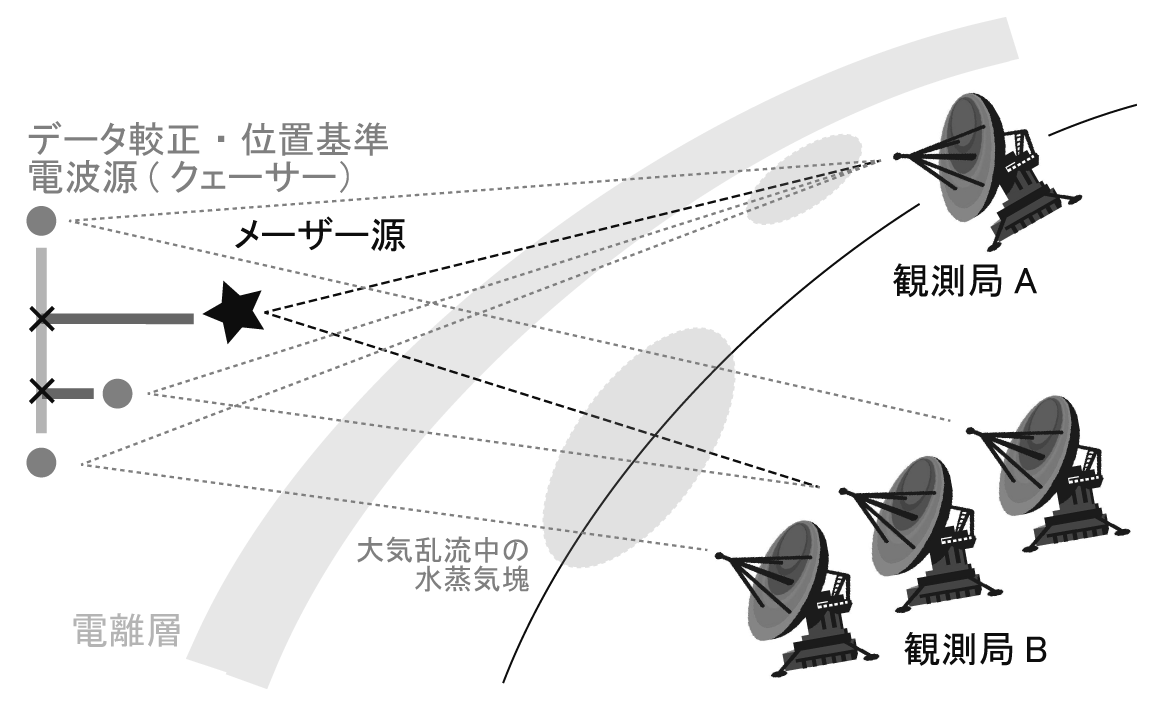
\includegraphics[width=0.7\linewidth]{astrometry/VLBI_calibration.eps}
\end{center}
\caption{SKA測量におけるVLBI観測モード。単一望遠鏡視野が長波長帯では多くなるので、
観測測量対象天体とその同じ単一望遠鏡視野に入る参照電波源とを同時に観測する手法が主流となる。
ただし、電離層による影響の仰角依存性に対しても計測してそれをデータ校正に利用する必要があるため、
測量天体からやや離れた参照源も観測する必要がある。従って、それぞれのVLBI局は複数視野
(最低4方向)を持つことが要求される。}\label{c7.s2.f3}
\end{figure}

\setcounter{subsection}{0}\subsection{VLBI観測装置}\label{c7.s2.ss1}
SKAにおけるVLBI観測向きの仕様は、
{\it SKA PHASE 1 VLBI CLARIFICATION ECP 140008 ANALYSIS DOCUMENT}\citep{SKA-VLBI}や
{\it SKA PHASE 1 SYSTEM (LEVEL 1) REQUIREMENTS SPECIFICATION}\citep{SKA1-requirement}にまとめられており、
さらにSKA Science Bookでも該当する内容が見られる\citep{Paragi...2015}。一般に、低い周波数ほど角分解能が低下するため、
より高い信号雑音比での電波源の検出と、参照電波源と測量対象電波源とを同一視野に入れた電波源位置計測
``in-beam astrometry"による地球大気による位置揺らぎの完全除去が必要になる(図\ref{c7.s2.f3})。
このような電波源測量に必要な仕様も含めてまとめると、以下の通りである。

\paragraph{広帯域受信系(フィード及び受信機)}
広帯域受信は、単純に感度向上のためだけでなく、VLBIの場合は群遅延時間の残差を精度良く推定してデータ校正や天体位置計測
の精度を向上するためにも必要である。SKAの周波数バンドでは、電離層の影響が大きいため、
またパルサーの観測では大きなdispersion measureを持つ遠方パルサーを観測するためにも、
広帯域受信(1~GHz帯で300~MHz以上を想定)が必要とされている。さらに、
22~GHzや23~GHz帯にある水やアンモニアメーザーを観測する為には、
Band 5の帯域をさらに高い周波数まで拡張するか、まだ搭載が予定されていない高周波数帯の受信機を別途搭載する
(あるいはSKA-highを進める)必要がある。
ちなみにSKAの``dish"と呼ばれるパラボラアンテナの鏡面精度については、20~GHz程度まで観測できる仕様が考えられている。
また、フィード(給電部)や低雑音増幅器の設計が進み、それぞれ1--20~GHz、2--20~GHz の範囲をカバーするものが
考案・開発されている(e.g., \citealt{Dubrovka2010,Komiak2011,Ujihara2014})。

\paragraph{アンテナビーム}
SKAコア局及びリモート局は、口径15mのアンテナ群から構成されるはずである。口径が比較的小さいので、視野が広くとれる。
SKA1-surveyでは、Phase Array Feed (PAF)を導入することにより、30平方度をカバーする。
このようにして、複数電波源の相対離角を非常に精密に測定することを可能とする。

\paragraph{周波数標準装置}
現在使われている水素メーザー周波数標準程度の高い周波数安定度の信号・時刻符号生成装置を各観測局に配置する必要がある。
1つの周波数標準の信号を安定して届けられる範囲は、現在100~km以内と言われている
\footnote{2011年5月にパースで行われたSKA及びVLBIに関するワークショップでなされた講演より。
現在においてこれを実現するためには、専用のダークファイバーの敷設が必要。}。

\paragraph{複数アンテナ受信信号の加算--- phase-up}
複数アンテナで受信された信号を加算(phase-up)していくことによって感度が向上する。しかし逆に、
アンテナ配置間隔に従って視野が狭くなっていき、本来単一望遠鏡視野で得られる視野を隅々まで観測できなくなる。
そこでSKAコア局とリモート局それぞれでは、
単一望遠鏡視野内で複数視野(遅延追尾位相中心)をとるべく個々の視野に対するphased-upの演算を行う。
そのために、受信信号が速やかに高速アナログ・デジタル変換され、デジタル信号でこの演算を行う。
さらに大きな離隔をカバーする場合は、局内アンテナ群を視野の数だけ分割して同時複数視野をとることもある。
最低4方向のビーム合成を行えば、大角度での位置天文・測地観測を通して基線ベクトルの向きと大きさ、
電波源座標を同時に求めることができる
\footnote
{1990年代前半までに提案されていたVERA(VLBI for Earth Rotation and Astrometry、現在のVERAの前身となるアイデア)では
この原理を元に設計されていた。20年の時を経てこのアイデアが復活したことを、ここに書き留めておきたい。}。
このような大離角複視野位置天文観測は、同一視野に参照電波源と測量対象天体が入らない場合の測量、
高精度電波座標系の構築、地球大気(電離層・対流層乾燥大気・水蒸気)
による影響の仰角依存性の推定とその除去にも利用される。

\paragraph{受信信号記録装置}
複数のアンテナ群から、あるいは複数の遅延追尾位相中心で処理された信号を、一旦メディア(多分ハードディスク)
上に記録する必要がある。広帯域化を進める上で、記録装置を含むデジタル信号処理の高速化が一番の課題だと言える
\footnote{周波数変換を行わずに受信信号をいきなりアナログ--デジタル変換するダイレクトサンプリングの開発が進んでいる
(e.g., \citealt{2012ivs..conf...91O})。}。
SKA1では500~MHz帯域記録を想定しているので、1視野につき記録速度は2~Gbps (ギガビット/秒)
でなければならない。後日、全観測局のデータ(24時間観測につき約170~TB)を持ち寄り相関処理を実施する。
その際は光通信ケーブルで伝送しなければならない。

\paragraph{高精度天体位置計測用校正データ}
VERAで用いられているようなGPSを用いた天頂帯域遅延残差の推定が各観測局で行われる必要がある
\footnote
{気象観測点データに基づく校正手法も開発されつつあるが、SKA局周辺を密に観測点で埋めることは当面考えられない。}。
また、定期的な測地VLBI観測により観測局の座標も1~cm程度では決定しなければならない。
地球回転パラメータ\footnote{Earth Orientation Parameters を指し、
地球自転の軸の向きやグリニッジ子午線の基準時刻における方向を表す。}
はVGOS(VLBI2010 Global Observing System)観測網で即座に決定されるはずである。
\\

VLBIデータ校正は、最も感度の高いコア局とリモート局とを結ぶ基線を用いて、各リモート局ごとに行うべきである。
そのためには、フリンジ位相の変動が小さい間(コヒーレンス時間)の間に、校正用(参照)電波源が検出できなければならない。
コア局--リモート局が成す基線で達成できる感度(10-$σ$ノイズレベル)は、以下の通りである。
\begin{equation}
S_{\rm min} = R_{\rm SN}\frac{\sqrt{SEFD_{\rm core}SEFD_{\rm remote}}}{\sqrt{2\Delta\nu\tau}}\approx 
0.55\frac{\sqrt{[SEFD_{\rm core}/{\rm 3~Jy}][SEFD_{\rm remote}/{\rm 100~Jy}]}}{\sqrt{[\tau/100~s]}} [{\rm mJy}]
\label{eq:baseline-sensitivity}
\end{equation}

\noindent
ここで、$R_{\rm SN}=10$は信号--雑音比で、$SEFD$とはsystem equivalent flux density [Jy]でいわゆる望遠鏡感度の指標であり、
$\Delta\nu\approx 5\times 10^8$[Hz](参照電波源など連続波源の場合)は観測帯域幅、$\tau$は積分時間
(ここではコヒーレンス時間)である。

一方測量対象天体の電波像上における検出感度については、
近似的にはコア局--リモート局が成す基線の数($=$リモート局の数)$N_{\rm base}$と総積分時間$T_{\rm total}$
から算出できる\footnote
{リモート局同士で成す基線も含めると、感度が1.7倍程度まで改善される($N_{\rm base}=$40の場合)。}
(下記計算ではメーザー輝線を想定)。
\begin{equation}
S_{\rm line} = S_{\rm min, \Delta t}\sqrt{\frac{\Delta t}{T_{\rm total}}}\frac{1}{\sqrt{N_{\rm base}}}
\approx 
16\frac{\sqrt{[SEFD_{\rm core}/{\rm 3~Jy}][SEFD_{\rm remote}/{\rm 100~Jy}]}}
{\sqrt{[\Delta\nu/{\rm 10~kHz}])[T_{\rm total}/{\rm 600~s]})[N_{\rm base}/{\rm 10}]}}[{\rm mJy}]
\label{eq:array-sensitivity}
\end{equation}

\noindent
式\ref{eq:accuracy}にあるように、高精度測量の対象は非常に高い信号--雑音比($>$100)で検出される必要があるので、
例えば、天の川銀河中のメーザー源の測量は
0.1~Jy以上のメーザー源に限られることになる。しかしこのようなSKA1の仕様でも、
現状の1/10倍暗いメーザー源も測量対象になる。
感度及び測量効率(如何に多くの天体を特定期間内に測量するのか)の計算に必要な各周波数バンドにおけるパラメータの概数を、
表\ref{c7.s2.t1}にまとめておく。

\begin{table}[h]
\caption{SKA-midで想定される感度と関連パラメータ。\citet{SKA1-BD}等を参照。}\label{c7.s2.t1}
\begin{center}
\vspace{-3mm}
\begin{tabular}{lrrr} \hline\hline
 & \multicolumn{3}{c}{SKA-mid bands} \\
 & SKA-mid Band 2 & SKA1-survey PAF Band 2 & Band 5 \\ \hline 
周波数範囲 &  0.95--1.76~GHz & 0.65--1.67~GHz & 4.6--13.8~GHz \\
コヒーレンス時間\footnotemark[1] & 200~s & 200~s & 100~s \\
スペクトル分解能 $\Delta \nu$ & 3.9~kHz & 1.95~kHz & 9.7~kHz \\
単一素子アンテナ視野半径 & 0.49$^{\circ}$ & 2.4$^{\circ}$ & 0.07$^{\circ}$ \\
$SEFD_{\rm core,SKA1}$\footnotemark[2] & 3.0 Jy & 7.0 Jy & 4.0 Jy \\
$SEFD_{\rm core,SKA2}$\footnotemark[3] & 1.0 Jy & --- & 1.3 Jy \\
$SEFD_{\rm remote,2015}$\footnotemark[4] & 100 Jy & 100 Jy & 390 Jy \\
$SEFD_{\rm remote,SKA2}$\footnotemark[5] & 16 Jy & --- & 21 Jy \\
$N_{\rm base, SKA2}$\footnotemark[6] & 40 & --- & 40 \\
\hline
\end{tabular}
\end{center}
\vspace{-3mm}\noindent
\footnotemark[1]代表的な値で、実際の解析は2--3倍長い値を採用できる。\\
\footnotemark[2]SKA1-midではコア局全体の70\%(望遠鏡配置中心の100~km以内)のアンテナ利用を想定。\\
\footnotemark[3]SKA1の10倍スケールのSKA2を想定し、その全アンテナの30\%の利用を想定。\\
\footnotemark[4]Band 2 では口径60~m級、Band 5では口径30~m級の2015年時点での既存電波望遠鏡(開口能率50\%、
システム雑音温度50~K程度)を想定。 \\
\footnotemark[5]口径15m鏡25台から成るSKA2リモート局(アンテナ仕様はSKA1のものと同じ)を想定。 \\
\footnotemark[6]SKA2アンテナの約半分(1000台)を使ってSKA2リモート局を構成する場合を想定。
\end{table}

\setcounter{subsection}{1}\subsection{VLBI観測局配置}\label{c7.s2.ss2}
高精度電波源位置計測にとって適切なVLBI観測局の配置については、具体的なシミュレーションをして定量的に
確認する必要があるが、リモート局の誘致・設置には様々な要因が関わってくる。リモート局の数は、
SKA2においてリモート局に配置する約1000台のアンテナに対して1局当り何台配置するかで基本的には決まる。
SKAOから提供されているテンプレートでは、アフリカ周辺にリモート局を約30カ所配置することになっている。

図\ref{c7.s2.f4}では現状で想定されるリモート局の配置を示している。
SKA-mid の周波数帯(0.4--15~GHz)では南アフリカから欧州・インド・
豪州にわたるVLBI観測網を想定する。SKA1-survey の周波数帯(0.4--4.0~GHz)では、それらに加えて、
日本も含むアジアのアンテナ群も含まれる。既存の電波望遠鏡についても、
2030年頃まで運用される可能性のあるものについても含めることができるだろう。
ちなみに欧州VLBI観測網(EVN)は、SKAのpathfinder として定義されている。
日本の電波望遠鏡インフラが日本とほぼ同じ経度にある豪州に展開される
SKA1-surveyとともに電波源測量に参加する場合は、
SKA1-surveyの帯域での測量を主に想定しておかなければならないだろう。

いずれにしても、想定されるリモート局配置によってどのように天体位置計測の精度が変わるのか、
数値シミュレーションによって調べる必要があるが、まだそれは系統的には行われていないようである。

\begin{figure}[t]
\includegraphics[width=0.425\linewidth]{astrometry/SKASA_stations_2011.eps}
\includegraphics[width=0.575\linewidth]{astrometry/SKA_and_GVN.eps}
\caption{SKA2や現行アストロメトリ精度推定シミュレーションで想定するVLBI観測局位置。
SKA建設地(南アフリカ及びオーストラリア西部)にあるコア局内アンテナ群(全体の50\%の集光面積)は
1局とみなす。それに加えて、SKAリモート局(アフリカ諸国、左図、参照URL: http://www.ska.ac.za)
や2030年頃まで実在する電波望遠鏡群を考慮している(右図)。日本国内にも1カ所想定している。}\label{c7.s2.f4}
\end{figure}

\setcounter{subsection}{2}\subsection{データ校正法・電波源位置計測法}\label{c7.s2.ss3}

VLBIデータの処理のうち、データ(フリンジビジビリティ)校正については、
現状VERAやVLBAなどで得られたデータに対して用いられているものとそれほど大きな違いはないだろう。
ただし、非常に高い信号--雑音比を電波像上で実現する為には、系統的誤差を従来以上に軽減し、
かつ、より高い電波画質が求められる。
電離層など地球大気に対する補正については、時間間隔を小さくして位相揺らぎを止めるだけでなく、
in-beam astrometry においても仰角に加えて方位角に対する微小の差分も考慮したものが必要である。
そのためにも、様々な仰角にある校正用電波源を複数個同時に観測する必要があるだろう(図\ref{c7.s2.f3})。
現在、VLBAを使った星周OHメーザー源の測量を進めており、このような手法の実効性の検証を進めているところである。

得られた電波画像については、高精度位置計測に向けてさらに詳細な分析が必要となる。
JASMINE等現在検討されている宇宙空間飛翔体による光赤外線位置天文では(例えば\citealt{2012A&A...538A..78L})、
観測装置の特性と星の位置情報を表すパラメータとを同時に解くことが行われている。
前者については、光学系で結像される星像の形状を詳細にモデル化し、
観測装置上で1/100 pixelオーダーで星像中心を導出し、その上で、像面の変形、
検出器の特性や放射線による特性の変化、読み出しエレクトロニクスの特性、
さらに飛翔体の軌道や姿勢を十分な精度でモデル化することを指す。
これと後者とを同時に解く事により、星の年周視差や固有運動などを精密に推定するのである。
一方電波画像による位置天文では、画像処理にさらなる改良のアイデア
(例えば「粗性モデリング」の手法、\citealt{2014PASJ...66...95H})が検討されているが、
位置天文情報は像合成に必要な情報とは別途のものとして取り扱われることが検討されてきた。
しかし、光赤外位置天文の手法同様に電波源位置計測においても、
観測装置起因のビジビリティ校正項、地球物理学的パラメータ(プレート運動による観測局の移動、
大気による超過遅延残差)そして天体位置情報のパラメータを同時に解くことを検討すべきかもしれない。

さらに、輝度中心(光学中心)を天体位置の指標としているところに、
光赤外及び電波位置天文共に大きな課題が残っている。
もしこれが天体の重心とずれている場合、モデル化誤差が発生する。連星系、
重力レンズ効果を受けた星などは、統計的に検出して、座標系構築に用いる星
からはじく必要がある。観測数$N$を増やした時に推定残差が$\sqrt{N}$に反比例して減ってゆかない場合は、
何らかのモデル化誤差が存在することが予想される。また、例えば超巨星は半径が1AU程度に及ぶものもあるが、
この巨星の表面に黒点があれば、これもバイアス要因となる。
このような天体由来の誤差要因について、メーザー源位置計測では既にその問題による影響が確認されている
(例えば\citealt{2014ApJ...787...54A})。個々のメーザー源は多数のメーザースポット群から成り立っている。
メーザー源の輝度分布から10\uas の精度で星の中心を正しく推定しているのはまず不可能である。
従って通常は、個々のメーザースポット毎に位置計測を行う。しかし、年周視差は複数スポットの動きを考慮した
モデルフィティングによって高精度で求められるが、メーザー源($=$星)そのものの固有運動を精度良く求めるためには、
メーザースポット群の三次元速度場を正確にモデル化してそれを解かなければならない。
さらに個々のスポットについても理想的な点源ではなく、
形状が長期間安定しているものを選んで年周視差計測に利用しなければならない。
一方、パルサーやYSOからの非熱的放射は、
点状にしか見えない星の本体から非常に近い場所からのスポット状放射なので、
一般相対論的効果が存在しても天体が孤立していれば、このような影響を無視することができる。

\setcounter{subsection}{3}\subsection{長波長帯における高精度天体位置計測の実現性}\label{c7.s2.ss4}
電波像上の信号--雑音比を向上させればより高い天体位置計測が実現するはずだが、
複数メーザースポットが同一VLBIビームに入る場合やリモート局数の数が限られている場合はその比は画像上の
dynamic rangeによって制限される。より多くの天体について測量するためには、
個々の天体の観測時間も短く制限しなければならない。従って、
達成できるdynamic range\footnote{画像上の輝度ピークのサイドローブなどを含む雑音に対する比。}
やメーザースポット群の構造による位置計測への影響の大きさは、
シミュレーションによる詳細な予測が必要である。

我々は現在、以上列記してきた事項を考慮して実現できる電波源位置計測の精度の評価を進めるべく、
シミュレーションソフトウェアの整備を進めているところである。
具体的には、ARIS(Astronomical Radio Interferometry Simulator, 
\citealt{2007PASJ...59..397A} )が擬似的に生成するVLBIビジビリティからAIPS(Astronomical 
Image Processing System)/ParselTonuge(AIPSを外部から操作するPythonスクリプトライブラリ)を
使って次々と電波像を合成し、得られる天体位置計測精度を統計的に調べる手法の開発を進めている。

\setcounter{subsection}{4}\subsection{測量用校正電波源}\label{c7.s2.ss5}

 前述の通り、低周波数バンドでの高精度測量では、測量目的天体と同じ望遠鏡視野に参照電波源が見えることが必須となる。
既存のVLBIデータ校正・位置参照用電波源のリスト\footnote{Leonid Petrov氏管理のHP、http://astrogeo.org}を参考にして、
測量目的天体のすぐ近くにこのような参照電波源がどのくらい存在するのか推定ができる。式\ref{eq:baseline-sensitivity}によれば、
1~mJy程度の電波源がSKA1では参照電波源として用いることができる。

図\ref{c7.s2.f4}及び\ref{c7.s2.f5}から、1~mJy以上の参照電波源の全天における総数を大雑把に推定できる。
QSOなどのRadio Loud な天体の総個数の推定\citet{SKA135}(図\ref{c7.s2.f5})で、
フラックス密度に対する度数頻度傾斜が得られている。これを採用して、精力的に電波源探査が進んでいる北天
(赤緯$-30^{\circ}$以北)の電波源に対して、累積度数頻度を1~mJyの方へ外挿することによって参照電波源の総数
を推定した(図\ref{c7.s2.f6})。その結果、
S帯(2.2~GHz)とX帯(8.4~GHz)とで全天にわたってそれぞれ約160 000個と130 000個の参照電波源が
存在し、SKAアンテナ視野(それぞれ0.75平方度、0.016平方度)当たり約2.9個と0.05個存在すると算出された。
これは、Band 2では何時でも測量目的天体と同じ望遠鏡視野に複数の参照電波源が見えることを意味する。
Band 5では、SKA1の間はアンテナ視野をコヒーレンス時間以内に切り替える必要があることを示唆する。

\begin{figure}[t]
\begin{minipage}{7.7cm}
\begin{center}
\includegraphics[width=0.75\linewidth]{astrometry/135_Memo_QSOs}
\end{center}
\vspace{-8mm}
\caption{SKAアンテナの視野に入る推定電波源数\citep{SKA135}。
QSOを含むRadio Loud源の度数頻度傾斜($N\propto S_{\nu}^{-0.9}$)を参考に、VLBI参照電波源の個数を推定する。}
\label{c7.s2.f5}
\end{minipage}
\hspace{5mm}
\begin{minipage}{7.5cm}
\includegraphics[width=1.0\linewidth]{astrometry/SKA_calibrators.eps}
\vspace{-8mm}
\caption{2014年12月時点で登録されている赤緯$-$30$^{\circ}$以北のVLBIデータ校正・位置参照用電波源の累積度数分布。
点線は図\ref{c7.s2.f4}の度数頻度傾斜と同じ傾斜を示し、それを使った外挿点から1~mJy (Log $F_{\rm correlated}{\rm [Jy]} = -3$)
よりも明るい電波源の総数を推定する。}
\label{c7.s2.f6}
\end{minipage}
\end{figure}

SKA1ではSKAコア局しか新規建設されないので、
既存電波望遠鏡と組み合わせてVLBI観測を行うことになる。大口径ほど感度が上がり、
測量対象天体のより近くに参照電波源が見つかり易くなるはずだが、
代わりに視野が狭くなって測量対象天体と同一視野に入る参照電波源数も減ってしまう。

実際に参照電波源として利用する為には、天球基準座標系内での正確な位置($\sigma<$1~mas)が必要である。
微弱な参照電波源については、当初その座標が正確には分からないが、
既知のQSOとの相対位置の計測が進めば座標の精度が向上するはずである。
ちなみに、天球座標系を構築する明るいQSOの位置精度は10~$\mu$asに達する。

\setcounter{subsection}{5}\subsection{天球電波座標系}\label{c7.s2.ss6}

現在、HIPPARCOS座標系と国際天球座標系(ICRF)との整合性の精度は0.5~mas程度\citep{1998A&A...331L..33F}であり、
また観測時期によってその値も異なる。光赤外位置天文ではGaiaが、
電波ではVERAやEVNが10~\uas の精度で天体位置計測を進めてそれぞれ位置天文カタログを構築している。
今後、これらカタログに共通に含まれる天体については数\uas 程度の精度で一致させることが、
目標の1つとして考えられる。しかし、10\uas の精度ではQSOはもはや不動点ではない。
電波源の輝度中心が必ずしも重心と一致するとは限らない。またその構造に変化があれば、
輝度中心は動くことになる\citep{2008IAUS..248..324B}。また電波の波長によっても、
光学的厚みの違いによってAGNジェットの見えている場所が異なる
(「コア・シフト」効果、 \citealt{2011Nature...477...185H})。Gaiaでは、
50万個のQSOから統計的に0.3\uas ~yr$^{-1}$の無回転座標を得ることを計画しているが、
このような多数のQSOによる統計処理、あるいはQSOを構成するジェットの構造に立ち入った精密なモデル化をしなければ、
QSOを不動点として座標を構築することはできない(\ref{c7.s3.ss5}節の銀河光行差も参照のこと)。

%%%%%%%%%%%%%%%%%%%%%%%%%%%%%%%%%%%%%%%%%%%%%%%
%\newpage
\setcounter{section}{2}\section{国際SKAのサイエンス}\label{c7.s3}

国際SKA研究者コミュニティーがSKAによる天体位置計測に基づくサイエンスの検討を深めている場は、
当初主にPulsar Science Teamに限られていた。VLBIコミュニティーによるこの方面についての本格的検討は、
\citet{SKA135}による提案によって始まったと言える。その後、
SKAによる電波源測量に基づくサイエンスについての議論が2014年5月に行われ\footnote
{Lorentz Center Workshop --- Galactic Science with the SKA \& Its Pathfinders ---, on 2014 May 19--23\\
URL: http://www.lorentzcenter.nl/lc/web/2014/631/info.php3?wsid=631\&venue=Oort} 、
その成果の一部がSKA Science Bookにまとめられている\citep{Green...2014}。
これらの議論では、現行のVLBI測量プロジェクト(VERA, VLBA, EVN, LBA)での成果を踏まえているので、
この節でこれらについても概覧しておく(例えば、\citealt{2014ARA&A..52..339R})。
また日本においても、\citet{SKA135}以前から幾つかの重要課題が提唱されているので、
この章で整理しておく。さらに、高精度天球基準座標系の構築(第\ref{c7.s2.ss6}節)の副産物として、
幾つかの重要な科学的課題へのアプローチが考えられることにも触れておきたい。

\setcounter{subsection}{0}\subsection{パルサーに対する年周視差・固有運動計測}\label{c7.s3.ss1}

パルサーによる科学研究の詳細は、第\ref{pulsar}章で既に取り扱われている。
そこでは主に、10~nsの精度でパルス到達時間の周期(pulse times-of-arrival, TOAs)を計測し(パルサータイミング)、
そこから展開される科学的課題について論じられている。
100 000個程度のパルサーの検出と10 000個程度のパルサー位置計測がなされることが期待されている。

ここで特筆したいのは以下の2点である。
1つは、パルサータイミングだけではパルサーの絶対座標及び固有運動が求まらないという点である
\footnote{パルサーの固有運動計測法が開発されている\citep{2003ASPC..302..215H}が、
この手法と独立して直接測定する必要もある。}。
パルサーに関するほとんどのパラメータはTOAsの時間変調計測に基づいているが、
電離した星間物質の中をパルサーが移動する時に発生するパルスの広がりやパルス強度の変調の詳細を明らかにするためには、
パルスの固有運動の情報が必要である。またそれらの把握は、
パルサータイミングを利用した長周期重力波の検出の精度を向上させるものと期待されている。
そのため、VLBI観測に基づく固有運動の直接計測は重要な課題である。

もう1つは、パルサータイミングの年周的変調を利用すると、撮像を通した電波源位置計測よりも高精度で年周視差を計測できるが
\citep{2011A&A...528A.108S}、
10年未満の計測期間の場合は(VLBI観測による)撮像に基づく手法の方が精度が高く、
より短期間でより多くのパルサーを測量対象にすることができることである。
年周視差変調のピークになる期間だけ位置計測をすれば済むので、観測所要時間も遥かに短くて済む。
天の川銀河内の多数メーザー源との位置比較(第\ref{c7.s3.ss2}節)を行うのであれば、この手法が重宝されるべきであろう。

\begin{figure}[t]
\includegraphics[width=1.0\linewidth]{astrometry/SKA_pulsars_simulation_2011.eps} \vspace*{-3mm}
\caption{パルサータイミングに対するシミュレーション\citep{2011A&A...528A.108S}。左図:黄道座標の極方向で200~pc先に
あるパルサーに対する疑似データ。SKAで期待される$\sigma\approx$10~nsの誤差を挿入している。
固有運動による直線的なTOA残差を差し引いた残りがここで表示されているが、年周視差による1年周期の変調が見られる。
右図:様々な黄緯にあるパルサーに対して期待される年周視差決定精度。細線と太線はそれぞれ5年間、10年間の
パルサータイミングの結果を示す(タイミング観測は2週間間隔)。}
\label{c7.s3.f7}
\end{figure}


\setcounter{subsection}{1}\subsection{天の川渦状腕内部の詳細構造}\label{c7.s3.ss2}

VERA, VLBA, EVNなどを使った年周視差と永年固有運動の計測が、
主に\ch3oh (6.7~GHz, 12.2~GHz)及び\h2o メーザー源に対して2000年代以降系統的に行われている。
その結果、天の川銀河の内部構造の動力学的研究が飛躍的に進んだ。
その概要は\citet{2014ARA&A..52..339R}にまとめられている。
これらのメーザー源の大部分は、
可視光で明るく見えるOB型星のすぐ近傍にある大質量星形成領域に付随しており、
天の川銀河の骨格を成す薄い円盤に付随しつつ、かつ渦状腕の形状の良い指標とされている(図\ref{c7.s3.f8})。
上記VLBI計測が一通り目処がつく2020年頃までには、1000天体程度の測量が完了し、
天の川銀河の構造を決定付ける基本的な要素が正確に把握されるだろう。
最も基本的な物理量である天の川中心--太陽系間の距離$R_0$や太陽系に
おける銀河回転速度$\Theta_0$が1\%の精度で推定され、渦状腕の形状、特に、
はっきりと存在する腕の数や各腕における真円に対するピッチ角、などが精度良く推定されるだろう。
さらに、$R\leq$15~kpcにわたる外縁までの銀河回転曲線と、
その半径内での銀河質量分布も正確に把握されるはずである。

このような状況から次の段階へと進む事が期待されるSKA時代における天の川銀河の研究では、
以下の課題が重要になるだろう。

\begin{figure}[t]
\begin{minipage}{8cm}
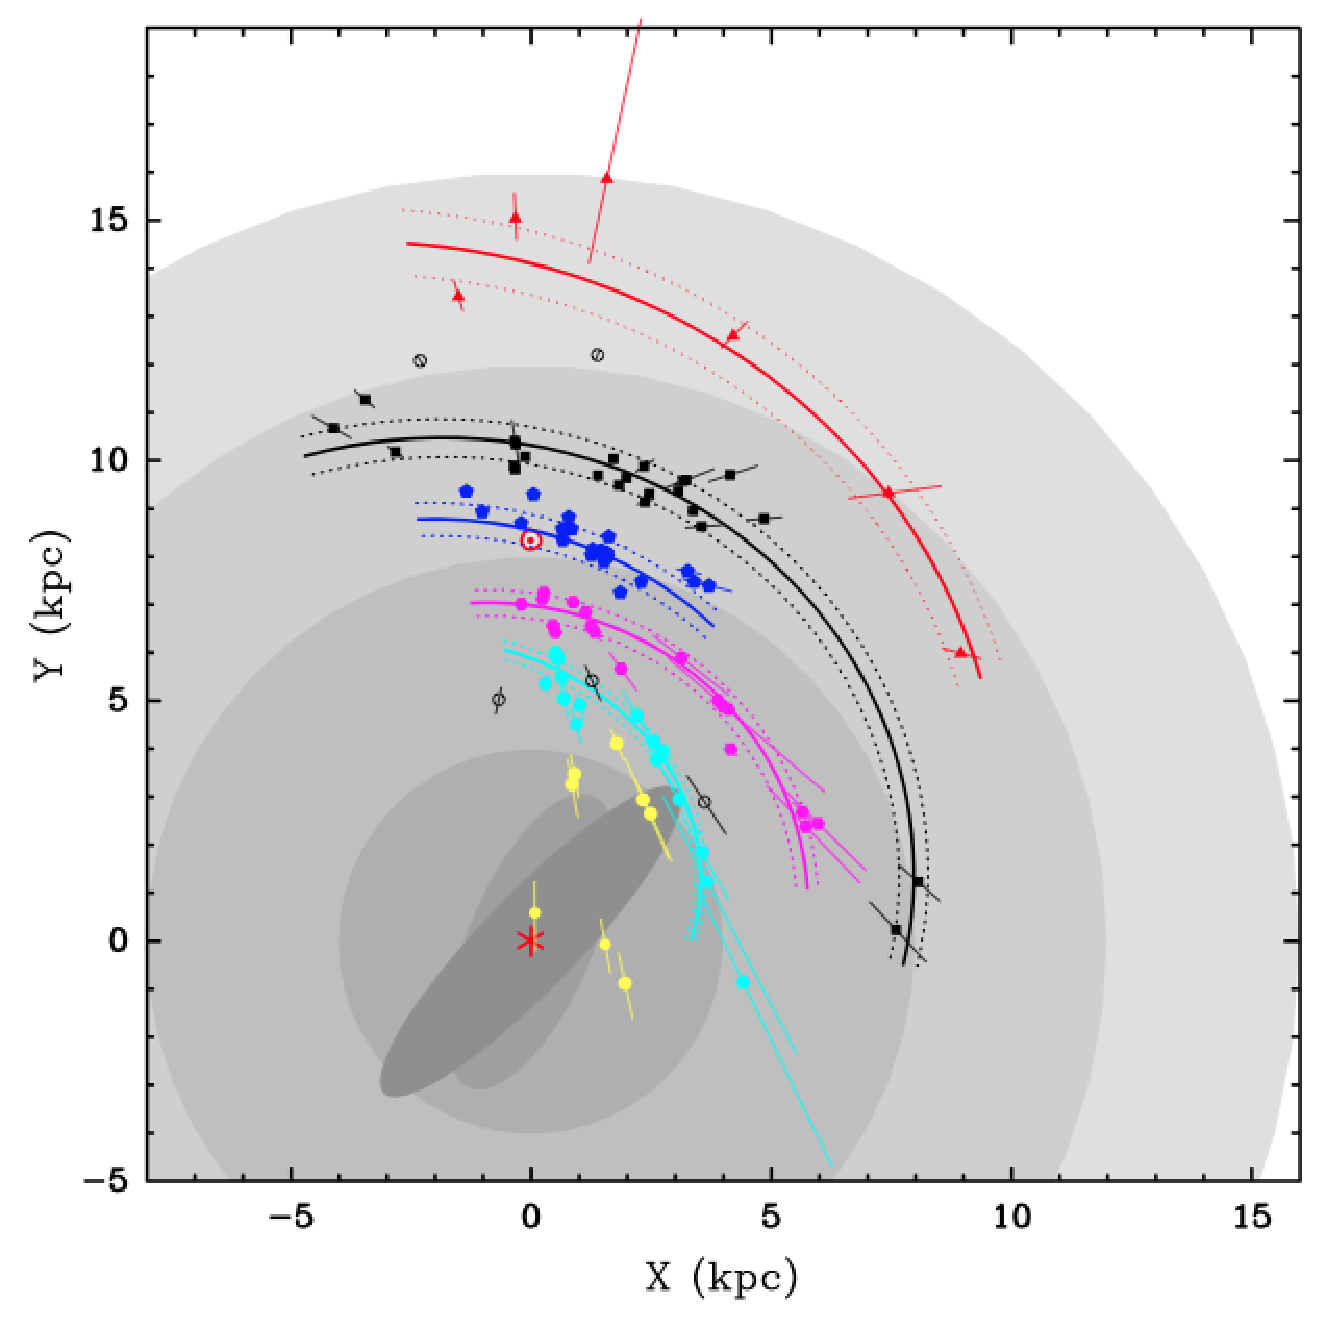
\includegraphics[width=0.9\linewidth]{astrometry/Reid_2014.eps} \vspace*{-3mm}
\caption{VLBIを使った測量で求められた天の川銀河円盤内のメーザー源の分布\citep{2014ApJ...783..130R}。
色付実線は渦状腕の形状を表し、異なる色がそれぞれ異なる渦状腕への所属を示す。 }
\label{c7.s3.f8}
\end{minipage}
\hspace{5mm}
\begin{minipage}{8cm}
\hspace*{-8mm}
\includegraphics[width=1.1\linewidth]{astrometry/Barros_2013_RotCurv.eps} \vspace*{-7mm}
\caption{天の川銀河の回転曲線(赤線)と渦状腕の形状パターン速度(斜め点線)\citep{2013MNRAS.435.2299B} 。
緑線は、ペルセウス腕と局部腕の間の密度ギャップを仮定した際にそれが作り出す回転曲線の凹みを示す。
2つの縦破線はCorotation radius の推定値を示す。}
\label{c7.s3.f9}
\end{minipage}
\end{figure}

\paragraph{天の川銀河南天域にわたる基本的構造の把握}
現在のメーザー源位置計測のほとんどでは、北半球にあるVLBI装置を使って北天を重点に測量が行われている。
視野や技術的限界のため、天の川銀河中心方向の年周視差測量までは可能だが、
銀河中心の向こう側の広大な領域がほぼ手付かずに残っている。
南半球に展開されるSKAでは、南天で銀河中心の向こう側にも手が届くようになる。
これにより、この方面での腕構造の様子や、銀河中心に存在するSgr~A*に対する銀河全体の
軸対称性が把握できるだろう。これは、天の川銀河基本物理量に対する系統的誤差を減じ、
さらなる高精度推定につながるものである。

\paragraph{Spiral arm tomography}
渦状腕の形成と形状維持については、長らく「密度波理論」が提唱されてきた\citep{1964ApJ...140..646L}。
渦状腕が星の銀河回転と共に移動していくのではなく、
同じ場所で定常的に「密度波」が立ってそこをガスが通過するたびに星形成が生じるという考え方である。
一方で最近、渦状腕は定常的な存在でなく、局所的な重力ポテンシャルの溝が銀河円盤内であちこちにできてそこに
渦状腕が発達するというモデルも提唱されている\citep{2009ApJ...706..471B} 。
銀河回転曲線は図\ref{c7.s3.f9}のように与えられているが、密度波理論と組み合わせて考えた場合、
(剛体回転すると予想される)渦状腕の形状パターン速度$\Omega_{\rm p}$と星・ガスの回転速度$\Theta$
が一致する銀河半径(corotation radius, $R_{\rm cr}$)よりも銀河中心側($R<R_{\rm cr}$)
ではパターン移動方向の上流から下流、
外縁側($R>R_{\rm cr}$)ででは下流から上流に向かってガスが流れ込むことになる。
この順序で星がない分子ガス雲、若い星形成領域、発達した星団などが見られるはずである。
現在のVLBI測量ではkpcを超えるスケールについては若い星形成領域の分布しか把握できない。
しかし、SKA1とのVLBI観測では、近傍星形成領域の前主系列星に対するVLBI測量
(e.g. \citealt{2013IAUS..289...36L} )の手法がkpcスケールにまで拡張されることが期待される。
また、非熱的放射を利用してOB型星を中心に他の進化段階にある星についても測距が可能になるはずである。
このように直接測量される天体に加えて、HII領域など、運動学的方法でしか距離を推定できない天体についても、
より正確に距離推定が可能となる。これらの天体とほぼ同じ方向に見えて測量された複数の天体に対して、
手前あるいは奥に存在するかどうかについて、電波スペクトル線(再結合線など)の輝線・吸収線の有無によって
判別ができるようになるのである。渦状腕中の進化段階毎の星々の分布の系列を判別するためには、
天体距離推定誤差$\sigma_{D}$に対して以下の条件を満たす必要がある。
\begin{equation}
\left|\Theta - \Omega_{\rm p}R\right| \times t_{\rm evolve}>\sigma_D
\label{eq:density-wave}
\end{equation}

\noindent ここで$t_{\rm evolve}$ は、星が主系列星になる前に測量可能な電波を放射する期間である。
\ch3oh /\h2o メーザー源だけを考えた場合、$t_{\rm evolve}\leq 10^6$~yr 程度で、
$\left|\Theta - \Omega_{\rm p}\right| \sim$20\kms 程度であれば式\ref{eq:density-wave}左辺は20~pc程度となる。
これは、2~kpc先で1\%程度の精度で天体距離を推定できれば、上記のような分布系列を把握できることになる。
SKAでは後述するOHメーザー源やH{\rm II}領域の距離推定も多数実施できるはずで、
このようなトモグラフィー的な手法が実現することが期待される。

\begin{figure}[t]
\begin{center}
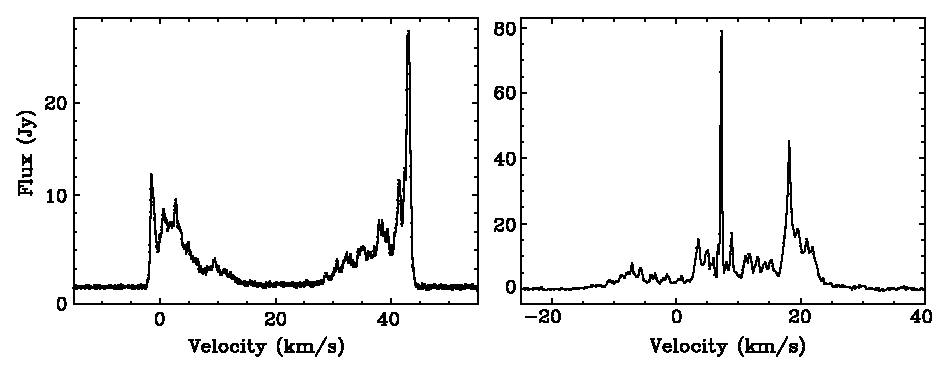
\includegraphics[width=1.0\linewidth]{astrometry/OH_spectra_Etoka.eps}
\end{center}
\vspace{-7mm}
\caption{典型的なOHメーザーのスペクトル(\citealt{Etoka...2014}より抜粋)。左図:長周期変光星OH~16.1$-$0.2に見られる
1612~MHz メーザー。左図:星形成領域Orion KLに見られる1665~MHz メーザー。}\label{c7.s3.f10}
\vspace{3mm}
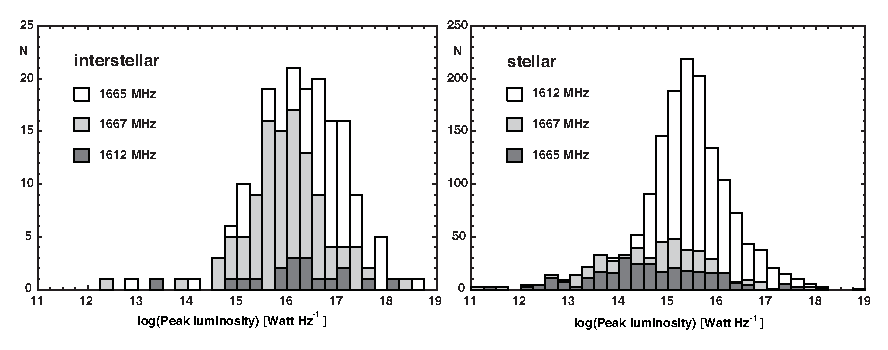
\includegraphics[width=1.0\linewidth]{astrometry/OH_LF_Etoka.eps}
\vspace{-7mm}
\caption{既知のOHメーザー源から導出されたOHメーザー光度関数(\citealt{Etoka...2014}より抜粋)。
左図、右図それぞれは、星形成領域及び進化末期星に付随するOHメーザー源のものを表す。}\label{c7.s3.f11}
\end{figure}

\begin{figure}[t]
\begin{center}
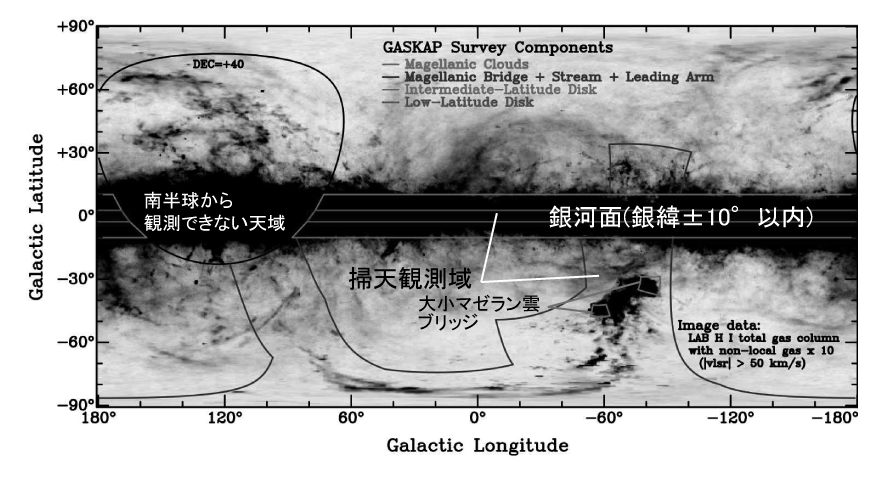
\includegraphics[width=1.0\linewidth]{astrometry/GASKAP_field.eps}
\end{center}
\vspace{-7mm}
\caption{銀河座標系上でのGASKAPの掃天範囲\citep{2013PASA...30....3D}。背景の灰色像は
角分解能約600\arcsec の掃天観測で得られたHI輝線の輝度分布 \citep{2010A&A...521A..17K}。
天の川銀河のバルジやハローはあまり含まれていないが、大小マゼラン銀河を含む広大な範囲
が含まれる。}\label{c7.s4.f12}
\end{figure}

\setcounter{subsection}{2}\subsection{OHメーザー源に対する位置計測と天の川銀河全体の構造の把握}\label{c7.s3.ss3}
SKAの観測周波数範囲には多数のOHメーザー輝線が含まれる。代表的な明るい輝線は、1612, 1665, 1667(以上Band 2), 
6031, 6035, 13341(以上Band 5) MHzに存在する。その中でも、主にAGB(漸近巨星枝)及び後AGB星に付随する
1612~MHzメーザーと主に大質量星形成領域に付随する1665, 1667~MHzメーザー、
一部の超新星残骸に見られる1720~MHz OHメーザーの探査が精力的に行われてきた。
1612~MHz及び1665~MHz OHメーザーで典型的に見られるスペクトルを図\ref{c7.s3.f10}に示す。
前者のスペクトルは基本的にはダブルピークを示し、そこから、
ほぼ球対称に放射状に一定速度で膨張する星周ガス縁の外縁部にメーザー放射源が付随することが伺える。
一方後者のスペクトルは、メーザー放射視線速度範囲の中央付近に見られる複数の鋭いピーク以外にも多数のピークが見られ、
生まれたての大質量星からの星風やそれ周辺ガス雲との相互作用が見られる領域など、
星形成領域の広い範囲にメーザー放射領域が存在することが伺える。

このようなOHメーザー源のVLBI観測は、\h2o、\ch3oh メーザーのものと並んで、星形成過程や恒星質量放出に関わる星間、
星周ガスの三次元運動の把握につながる重要な手法である。また、年周視差や固有運動の測定対象にもなる。
\h2o、\ch3oh メーザー源は主に天の川銀河の「薄い円盤」に集中しているのに対し(第\ref{c7.s3.ss2}節)、
AGB/後AGB星に付随する星周OHメーザー源は厚い円盤やバルジ、少数であろうがハロー(特に球状星団)
にも広く存在するはずである。
測量対象の数も一気に1--2桁増え、星間OHメーザー源測量によって天の川銀河の骨格の把握に大きく寄与するだけでなく、
星周OHメーザー源測量によって天の川銀河全体の力学構造の把握につながると期待される。
後者によるメーザー源の距離と固有運動の計測は同時に、
恒星から放出された物質が天の川銀河のどの範囲までにどの程度届くのかを把握することになるのである。
天の川銀河における恒星--星間空間における物質循環は、従来定性的に述べられていたに過ぎないが、
このような測定が物質循環の定量的評価へと研究の質を変貌させることになるはずである。

1612~MHz及び1665~MHz OHメーザーの光度関数(図\ref{c7.s3.f11})は、
約5000個に及ぶOHメーザー源データベース\citep{2012IAUS..287..254E}
から導出されている\cite{Etoka...2014} 。星間(1665~MHz)及び星周(1612~MHz)OHメーザー源サンプルの光度関数はそれぞれ
$L_{\nu}=10^{16}$ W$\cdot$Hz$^{-1}$、$2\times 10^{15}$~W$\cdot$Hz$^{-1}$にピークを持ち、
比較的単純なガウス型になっている。星周1612~MHz OHメーザー源の光度関数ピークは、
天の川銀河中心の距離($D\approx 8.3$~kpc)で1~Jy程度に対応する。

\citet{Etoka...2014}の試算によると、広視野を持つSKA1-surveyを用いれば、
10-$\sigma\sim$4~mJyの検出感度ならは143時間の積分で全天掃天観測を完了でき、
天の川銀河系外縁部のさらに微弱なメーザー源(1~mJy程度)の探査も53時間程度で完了できる。
大小マゼラン雲全域にわたる探査(10-$\sigma\sim$0.1~mJy)には2275時間掛かるが、現実的な数値であろう。
それ以遠の銀河に対する探査の場合は、視野が限られるがSKA1-midを使うことになる。
M33 の1平方度内を10-$\sigma\sim$0.05~mJyで探査するのに、160時間を要すると予想されている。
その前に2016年から予定されているGASKAP(Galactic ASKAP Spectral Line Survey)\citep{2013PASA...30....3D}
(図\ref{c7.s4.f12})では、天の川銀河面や大小マゼラン雲の広域をカバーする深い掃天観測が行われる。
その探査では、検出されるOHメーザー源の数は既知のメーザー源の数の2倍になるだろうと予想されている。
しかし、OHメーザー源の光度関数が低光度側に伸びていれば、
この予想を大きくはずれてより多数のメーザー源が検出されると期待される。
検出された1~mJy以上のメーザー源は、空間的に広がったものでない限り、全てがSKAによる測量対象になる。

現状では、OHメーザー源の年周視差計測に関する論文は3編しか存在しない
\citep{2000A&A...357..945V, 2003A&A...407..213V,2007A&A...472..547V}。
充分な角分解能を得ることが難しい上に、多くのメーザースポットが空間的に広がっている
\citep{2013ApJ...773..182I,2013ApJ...771...47I} 。
OHメーザー源に対する高精度測量には、充分に長いVLBI基線($>$3000~km)に加えて短基線も必要で、
非常に高い信号--雑音比($R_{\rm SN}>>$100)を得ると共に、正確な電離層補正が必須である。

比較的明るい天の川銀河内のOHメーザー源に対する測量ならば、広視野を一度に稼げるSKA1-surveyを
含むVLBI観測網によるものが効率が高いと期待される。
SKA1-surveyとアジア太平洋地域の60m級の大口径望遠鏡3台程度を組み合わせれば、
式\ref{eq:array-sensitivity}より440~mJy(100-$\sigma$)より明るいOHメーザー源が測量対象になり得る
(10分積分)。従って、上記掃天観測で検出されたOHメーザー源のうちわずかな割合で存在する明るいものしか
測量対象にならないだろう。しかし、SPLASH(Southern Parkes Large Area Survey in Hydoxyl)
\citep{2014MNRAS.439.1596D}の初期データを使って統計を試みると、
このような明るいメーザー源($S_{\nu}>$400~mJy)は天の川銀河面全体で約5000個存在すると推定された
(品野\& 今井私信)。これだけでも、VERAによる測量対象\h2oメーザー源の10倍の数にも及ぶのである。

\setcounter{subsection}{3}\subsection{局所銀河群(The Local Group) 中銀河の固有運動}\label{c7.s3.ss4}

マゼラン雲やM31(アンドロメダ銀河)も含めて、天の川銀河は局所銀河群(以下LG)のメンバーとなっている。
宇宙膨張を振り切って重力収縮しLGが形成されていくので、LGメンバー銀河、特に天の川銀河とM31の相対的な
直交速度は全エネルギー密度パラメータ$\Omega_{\rm 0}$ 
(下添字のゼロは現在の値を意味する)に依存すると示唆されている\citep{1990ApJ...362....1P,1994ApJ...429...43P}。
また、天の川銀河とM31が作るダークハローの中をこれらのLGメンバー銀河が周回しており、
これら銀河の軌道と形状の進化はダークハローの密度分布に依存する\citep{2001ApJ...559..754M}。
このように、M31やLGメンバー銀河について天の川銀河に対する三次元相対運動を把握できれば、
宇宙論パラメータやダークハロー密度分布の推定を通して、LGがどのような動力学構造をしているかを決めることができ、
そのメンバー銀河の力学進化を理解することにつながる。
しかし、視線方向の速度はドップラー効果の観測から容易に導かれる一方、
視線に垂直な方向の固有運動はとても微小な値になるので、挑戦的な天体位置計測となる。

最近、HST観測に基づいたM31の固有運動測定が行われた
\citep{2012ApJ...753....7S, 2012ApJ...753....9V, 2012ApJ...753....8V}。参照天体としては、
M31の背景にある多数の遠方銀河を用い、実質静止しているこれらの背景銀河のHSTイメージに対して、
M31のハロー、円盤の外側、ストリームの3つのフィールドにある恒星系の微小な動きを、
5年から7年の時間差がある2つの時刻で測定した。各フィールドで得られた固有運動の重み付き平均は、
M31の西と北方向へ($42.2 \pm 12.3$, $30.9 \pm 11.7$) $\mu$as~yr$^{-1}$であった。
これからM31の銀河系方向に垂直な方向の速度は、(銀河系の回転速度や太陽位置と運動の値を与えた上で)
$V_{\rm tan}=$17.0\kms(1$\sigma$の範囲では$V_{\rm tan} \le$ 34.3\kms)となった。
この結果は、M31がほぼ直線軌道に近い形で銀河系に近づくような運動をしていることを示唆しており、
今から40億年後には両者が合体する可能性が出てきた。

この観測結果は大きな反響があったが、M31の横断速度決定には依然不定性が残る。
一つは固有運動測定そのものにあり、HSTの狭い観測視野で設定された個別の観測フィールドでは、
各恒星の固有運動のばらつきが大きく、しかも(マゼラン雲の固有運動観測でも見られる振る舞いであるが)
観測時刻を2回より多くすると固有運動値が無視できない系統変化を示す。また、M31自体の内部運動
(回転、速度分散とその空間依存性)の補正が全く十分ではなく、
このためにはもっと多くの観測フィールドを設定してやらねばならない。
M31の横断速度決定の二つ目の不定性は、やはり我が銀河系そのものの回転速度や
太陽位置と運動速度の評価にある。

現在HSTだけでなく、\h2oや\ch3oh のメーザー源を標準光源としたLG銀河の固有運動の検出への挑戦が続いている。
M33($D\approx$800~kpc)では\h2o メーザー源を利用した固有運動$\mu\sim$30\uas ~yr$^{-1}$の検出に成功している
\citep{2005Sci...307.1440B} 。LGでは天の川銀河と双璧を成すM31についても、
最近\ch3oh \citep{2010ApJ...724L.158S}や\h2oメーザー源\citep{2011ApJ...732L...2D}
が発見されてからその固有運動計測が開始されている。従って、
SKAによってこれらのメーザー源を銀河の広い領域でかつ多数回に渡るアストロメトリ観測を遂行することにより、
LG銀河の正確な横断速度を決定することが可能となる。
また、SKA2の時代になると想定されるが、前節のように検出されたOHメーザー源も測量対象になり得る。

\setcounter{subsection}{4}\subsection{高精度天球基準座標系構築で生み出されるサイエンス}\label{c7.s3.ss5}

天球基準座標系を構築する多数の位置参照電波源の位置を高精度で長期観測すれば、
限られた天体数の位置計測では同定できなかった微小な位置変化をもたらす現象を捉えることができるようになる。

\paragraph{銀河光行差}
銀河系の太陽位置における回転速度の値は、これまで多く議論されてきたにも関わらず、
まだ収束した確定値になっていないのが現状である。その決定のためには、
銀河系内の様々な場所にあるメーザー源の固有運動と距離を正確に測定し、
それらを総合的に解析する方法が一般にとられている。
一方、太陽自身は天の川銀河の中を重力に引かれて加速度運動をしているので、
これにより遠方にあって静止して見えるはずの系外電波源に見かけの固有運動が発生する。
これはsecular abberation drift(永年光行差ドリフト)の効果によるもので、加速度中心に向かって収束し、
その反対側から発散するようなダイポール型の固有運動パターンが得られる。これを「銀河光行差」と呼ぶことがある。

銀河光行差による正味の固有運動量$\Delta \mu$は、銀河回転の速度を$V_c$、銀河系中心からの距離を$R_0$、
光速度を$c$とすると、$\Delta \mu = V_c^2/R_0 c$となり、これはおおよそ5 $\mu$as~yr$^{-1}$程度になる。
しかも、この値は加速度だけに依存しているので、太陽のいわゆる非円運動の効果を考慮せずに
独立に求めることができる。

\citet{2011A&A...529A..91T}は、555個の系外電波源に対して1990年から2010年にかけての位置の変化から固有運動パターンを求め、
$\Delta \mu = 6.4 \pm 1.5$ $\mu$as~yr$^{-1}$という値を導いた。
また、固有運動パターンは赤経、赤緯が(263$^{\circ}$, $-20^{\circ}$)方向に向かっており、天の川銀河中心方向に近い。
しかし、統計誤差や系統誤差はまだ大きいので、
SKAによって多数の系外銀河電波源に対する系統的な位置観測を長期に渡って遂行することが重要となる。これにより、
太陽位置での天の川銀河加速度(そして軌道速度)の値を正確に求めることができる。

\paragraph{天体位置計測上のマイクロレンズ現象}

可視光線測光観測では、手前の天体による重力レンズ効果によって背景の天体が一時的に増光される事例(測光的マイクロレンズ)
が多く確認され、手前の天体の特徴(連星系や惑星の有無も含む)の把握に大いに応用されてきた。しかしレンズ天体は軽く、
測光的マイクロレンズ現象は背景と手前の天体との離角が非常に小さくなければ測光観測では検出され辛く、
10$^{-1}$yr$^{-1}$の頻度程度となっている。

一方重力レンズ効果は、背景の天体の位置を一時的にずらすようにも働く。測光的マイクロレンズ現象は振幅が小さいが、
レンズ天体と背景点源との離角が多少離れていても検出されることが期待される。例えば天の川銀河バルジ方向の天体個数密度
では、10\uas 程度の効果ならば 毎年1 個の確率でICRF天体に対してレンズ効果が期待され、
1\uas レベルの精度での天球座標系構築は難しいとされている \citep{1997AJ....114.1508H} 。
さらに、パルサーも含む電波星の周辺に惑星が存在してもこの効果が期待される。


%%%%%%%%%%%%%%%%%%%%%%%%%%%%%%%%%%%%%%%%%%%%%%%
\setcounter{section}{3}\section{日本が狙うサイエンス}\label{c7.s4}

この章の冒頭にも述べた通り、天文時空計測の分野における日本がSKAを用いて狙うサイエンスは、
現在進行中のVERAや計画中のJASMINEが目指すサイエンスを基準に検討することが、ごく自然の流れである。
天の川銀河の「局所部」から天の川銀河「系」へ、天の川銀河の「現在」から天の川銀河の「歴史」へ、
局所的なものから大域的な天球座標系構築への貢献、等を想定することが求められる。
また(SKAから見る事ができない一部北天を除く)全天球面における測量は、
様々な研究分野とのシナジーを可能とする。その中で最も重要なシナジーは、既に述べたパルサー研究(\ref{c7.s3.ss1}節)
と突発天体研究(\ref{c7.s4.ss6}節、一部\ref{c7.s4.ss7}節)とのシナジーであると考える。

\setcounter{subsection}{0}\subsection{天の川銀河の薄い円盤と渦状腕のパターン速度の推定}\label{c7.s4.ss1}

この課題は既に\ref{c7.s3.ss2}節で解説しているが、日本のコミュニティーがこの課題で先頭を切るのであれば、
SKA1-surveyを含むアジア太平洋地域でVLBI観測網を展開し、
広視野を活かした星間OHメーザー源に対する測量を前面に押し出すことが考えられる。
豪州と日本はほぼ同じ経度なので、JAXA臼田64m鏡やNICT鹿島34m鏡などを利用して南北に長いVLBI基線を得ることができる。
中国の上海65m鏡やFAST、インドのGMRTを含めれば、東西にも長くしかも極めて感度の高いVLBI基線を獲得できる。

VERAをはじめ既存VLBI測量プロジェクトでは、
2020年頃までに北半球から見える約1000天体の\h2o, SiOメーザー源の測量が完了すると想定されている。
しかしその場合、渦状腕(いて座・局所・ペルセウス・外縁部腕)1本当たりのメーザー源多くても300天体程度に留まる。
ペルセウス腕の奥行きを1~kpc、北半球から見える長さを45~kpc程度と考え厚みを無視すると、
1~kpc四方の中にわずか7天体弱しかメーザー源が見当たらないことになる。50~pcメッシュ程度で測量データ点を得て、
spiral arm tomography (\ref{c7.s3.ss2}節参照)の手法で20~pc程度のメッシュで星形成領域の奥行き方向の相対位置
関係を把握することを目指すには、1~kpc四方の中に400天体のメーザー源が必要になる試算になる。

一方、SKA2の時代のmid-bandにおける測量について考察してみる。測量の主体として1.6~GHz帯のOHメーザー源を
考えた場合、15m鏡1000台から成るコア局と15m鏡36台から成る27カ所のリモート局を実現させることにより、
2015年時点のVERAの感度(\h2oメーザー源対象)に対して約80倍の基線感度と約300倍の検出感度を獲得
することになる。ただし、10000~kmの基線長を使っても角分解能が落ちることを考慮する必要がある。
しかしそれでも、同じ10~$\mu$as程度の位置計測精度での測量ならば、
VERAと同等の測量範囲を1/90の観測時間で完了する試算となる。
視野が広いので、同時に複数のメーザー源が測量される可能性を考えると、もっと測量の効率が上がる。
Spiral arm tomographyのための測量を実施する場合、1天体の測量に30分掛けて
(2年間掛けて3分間の観測を10回程度実施)\footnote
{望遠鏡運用の効率を考えると、1天体当たりの積分時間を極端に減らすことは好ましくない。
より遠方まで測量することを考えた方が生産的である。ここでは3分間程度の積分時間を想定する。}
約70 000天体測量することが想定され、年間240時間掛けて1000天体ずつ測量して7年弱でデータ取得が完了できるはずである。

\setcounter{subsection}{1}\subsection{天の川銀河の厚い円盤で見られる物質循環}\label{c7.s4.ss2}

進化末期星に付随する星周OHメーザー源(主に1612~MHz輝線)の銀河面垂直方向に沿った分布のスケール高度は約 600~pc
(SPLASH初期科学データ\citep{2014MNRAS.439.1596D}の処理結果より、品野\& 今井私信)であり、
天の川銀河の薄い円盤(スケール高度は約100~pc)よりもずっと厚いが厚い円盤
(約1000~pc)のものよりもやや薄いことが知られている。このように星周OHメーザー源は、
現在の天の川銀河における物質循環、特に恒星から放出された物質の星間空間への還元の主な担い手である中質量星
($1\:M_{\odot}\leq M_{\ast}\leq 8\:M_{\odot}$)の分布を反映しており、現在激しく進化末期に差し掛かった星々からの
大量物質放出の現場を反映する。

恒星からの大量物質放出の仕組みは、恒星物理学上重要であり、現在国内外で精力的に研究が進められている。
ここで問題なのは、このように恒星から放出された物質が何処へ行くのか、どこまでまき散らされるのかということである。
天の川銀河の厚い円盤まではほうり上げられるが、やがてマゼラン銀河など近傍の衛星銀河から降ってくる物質と混じって
共にやがて再び天の川銀河に薄い円盤に降り積もるはずである。淡く広がった星間ガスを成すこれら物質の位置と三次元運動
の把握は容易くないが、点源とみなせる星周OHメーザー源については、それらの情報をVLBI測量によって得られるはずである。
天の川銀河の厚い円盤の天体位置計測はGaiaが計測対象とするはずだが、星周OHメーザー源のように分厚い星周ガス縁に
覆われて中心星の位置が把握し辛い星々については、電波位置計測に向いているのである。

\setcounter{subsection}{2}\subsection{天の川銀河バルジ}\label{c7.s4.ss3}

 天の川銀河バルジには、その中心部に巨大ブラックホール(BH)が存在するが、
こうした巨大BHは銀河の中心部に不偏的に存在する。またバルジと巨大BHの質量比が、
バルジ質量 3 桁($10^{9}--10^{12} M_{\odot}$)に渡っておよそ1000:1となっている事が見出されており、
バルジと巨大BHは深く関係して形成、成長してきたと考えられる。従って、
天の川銀河のバルジを理解するにあたり、その中心部にある巨大BHも含めた理解が必要となる。
このBHの形成や成長過程については、角運動量損失によるバルジから銀河中心部へのガスや星、
中間質量BHといった物質の輸送メカニズム、すなわち物質供給機構の物理的機構を解明する事が重要である。
さらに銀河中心領域における分子雲(Central Molecular Zone, CMZ) (図\ref{c7.s4.f13})
内部におけるガスの集中や星形成などの活動の理解も合わせて重要である。
こうした角運動量の損失効果による物質供給機構は本質的にはバルジの力学構造、
すなわち重力ポテンシャルによって決定づけられる。従って、
天の川銀河中心領域における重力ポテンシャルを調べることは物質の供給機構の理解、
引いてはバルジと巨大BHの共進化を理解する上で必要不可欠である。

日本においては現在、VERAによるメーザー源位置天文が精力的に進められているが、
天の川銀河中心方向の仰角が低い為に観測時間が限られること、
撮像のために1観測当り数時間を要することから、
この方面にある位置計測が進められているメーザー源の数が非常に限られたもの($<10$)になっている。
従って、SKAが南天測量を精力的に進められる装置になることが強く望まれる。

ところで、現在国立天文台を中心に開発が進められている赤外線による位置天文観測衛星JASMINEは、
こうした銀河中心領域のポテンシャルの解析を行うべくこの方向の星に対する高精度位置計測と
恒星群の軌道解析を行う計画である。3段階からなるJASMINE計画のうち、第2段階にあたる小型JASMINE
(2020年頃)の観測領域は、CMZを含む図\ref{c7.s4.f14}に示す領域である。
この領域においては、約10$^{4}$個のバルジ星($H_{\rm W}<11.5$~mag、
ここで$H_{\rm W}$バンドとは1.1--1.7~$\mu$mの波長帯バンドを指す)
の年周視差($\sigma_{\Pi}\approx$10--20\uas )と固有運動($\sigma_{\mu}\approx$10--50\uas ~yr$^{-1}$)の計測を行う。
なおこの領域はGaiaではほとんど観測できない領域である。また最終段階では、バルジ全領域にわたり
約10$^{7}$個の星($K_{\rm W}<11$~mag)の測量を目指す。

これに対してSKAにおいては、
バルジだけでなく星間減光が激しい銀河中心最近傍に存在するOHメーザー源が主要測量対象になる。
銀河中心方向では、$K<9$~mag ($H_{\rm W}<11.5$~mag)を持つ長周期変光星に多数のSiOメーザー源が見つかっている
 \citep{2004PASJ...56..765D}。そのようなメーザー源には、0.5~Jy程度のOHメーザー源が一部付随している
 \citep{1998A&AS..128...35S, 1998A&A...329..991B}。
一方SKA1では$S_{\nu}\geq$0.1~Jy 程度の星周OHメーザー源が高精度位置計測の対象になる。よって、
この方面やバルジに付随する$K<10.7$~mag の変光星がSKA1での位置計測対象になり得る。
バルジ方向では約1000個のSiOメーザー源が検出されており\citep{2007IAUS..242..200D}、
その約半分がOHメーザー源だと推定される\citep{2002PASJ...54L..19I}。
星周OHメーザー源の光度はその光度関数(\ref{c7.s3}節)からほぼ一定と近似し、
バルジ方向に一様に分布していると考えると、
SKA1における位置計測の対象はバルジ方向で約5600天体に達すると推定される。
測量天体数においてはJASMINEのそれに比べてOHメーザー源のそれは遥かに小さいが、
$H_{\rm W}$バンドで測量する小型JASMINEのサンプル数に匹敵し、
サンプルの大部分は小型JASMINEと共通のものとなる。
よって、電波・赤外線測量において共通の対象天体については、
測量結果の整合性を確認して真の測量精度を把握することができる。

JASMINEとSKAとでは、測量対象の分布だけでなく主な測量対象となる恒星の質量分布が異なるはずで、
前者では中小質量の主系列星やAGB星、後者では比較的大質量のAGB星が主要対象になる。
従って、これら2つの位置天文ミッションは空間的にも時間的
(過去の星形成活動履歴の中で異なる年代に属する恒星群を成すという意味)にも相補的関係にあると考えられる。
こうして、総合的に銀河中心領域のポテンシャルの解明を進める事が可能となるはずである。
特に、OHメーザー源の一部が星形成領域に付随したものであることは特筆すべきことである。
赤外線とも共通して観測できる天体及びSKAでのみ観測可能な天体とを合わせて、
両者の運動を比較することができるだろう。そうすると、
星自身の運動とガスの運動が同じなのか違っているのか、もし違っていればその原因は何なのか、
についての理解が進むはずである。

\begin{figure}[t]
\begin{center}
\includegraphics[width=0.7\linewidth]{astrometry/CMZ.eps}
\end{center}
\vspace{-7mm}
\caption{銀河中心領域の分子雲(Central  Molecular Zone)  (@NRAO)。}
\label{c7.s4.f13}
\end{figure}

\begin{figure}[t]
\begin{minipage}{7.8cm}
\includegraphics[width=1.0\linewidth]{astrometry/JASMINE_field_lb.eps}
\vspace{-7mm}
\caption{赤外線位置天文観測衛星 小型JASMINEの観測領域。}
\label{c7.s4.f14}
\end{minipage}
\hspace{4mm}
\begin{minipage}{7.8cm}
\includegraphics[width=1.0\linewidth]{astrometry/JASMINE_field_xy.eps}
\vspace{-9mm}
\caption{銀河系中心領域における恒星軌道の様子。閉じる軌道(親軌道)のみ表示。}
\label{c7.s4.f15}
\end{minipage}
\end{figure}

 バルジ内の棒状構造においては、長軸方向が互いに異なるX1軌道とX2軌道が存在する。
これら軌道に付随する恒星群が互いに影響しあって、銀河中心部への物質輸送に重要な役割を演じる事が想定されているため、
星の軌道からそれらを理解する事が重要となっている(図\ref{c7.s4.f15})。

 天の川銀河の力学構造は、棒状構造のサイズや偏平度、更には星の回転速度、中心コア半径、
パターン速度といったパラメータでおよそ特徴づけられるが、
そうした特徴を兼ね備えた銀河力学モデルを構築することが考えられる。
また、その力学モデルからエネルギー$E$と角運動量$L$を与えられると、
その値における物質(星・ガス)の位相空間における質量の確率密度(位相分布関数$f(E,L)$)を作成することができる。

その一方で、観測より得られる星の位置や運動のデータがモデルから作成された分布関数にできるだけ従うように各種、
モデルパラメータを決定する。軌道の解析を行うのに都合が良いように以下のような数値計算を行う。
まず、ポテンシャルを仮定し、そこにいくつかの粒子を走らせる。
その走らせた粒子が作る密度分布から再現されるポテンシャルが初めに与えたポテンシャルに一致するように、
各粒子の重みを調整する(Self-consistent model)。これを利用した数値シミュレーションを用いて、
力学モデルの作成および小型JASMINEの疑似観測データを作成し銀河系の各種パラメータを導出したところ、
パラメータの値が99.7\%の信頼性で求められる事が確認されている。

\citet{2009ApJ...691.1525N}によれば、物質供給機構に関して内部バーが重要な役割を担っているが、
その内部バーの強さにはあまり依らずパターン速度が200~km~s$^{-1}$kpc$^{-1}$を超えると銀河中心領域への物質の供給が
スムーズに効率的に行われる事が示されている。
従ってパターン速度を定量的に求める事は物質供給機構の理解にとって非常に重要となる。
以上、重力ポテンシャルを定める事は物質の供給が今後どの程度おこるのかに定量的評価を与え、
さらにポテンシャルが分かっている事でバルジの星の未来の運動が分かることになり、この先の未来の予測が可能となる。

\setcounter{subsection}{3}\subsection{天の川--マゼラン銀河系の力学進化と物質進化}\label{c7.s4.ss4}

\begin{figure}[t]
\begin{center}
\includegraphics[width=0.8\linewidth]{astrometry/bekki_MCs.eps}
\end{center}
\vspace{-7mm}
\caption{Diaz and Bekki (2012)によるマゼラン流のシミュレーションと
その観測結果\citep{2003ApJ...586..170P}との比較。左図がシミュレーションによって
得られた中性水素ガスの柱密度分布を示し、右図が観測結果を示している。
シミュレーションモデルはバウンド軌道モデルに近く、過去三十億年に
マゼラン銀河系は天の川銀河を2回まわっている。彼らのモデルでは、
マゼラン流はその最初の周回運動の際、小マゼラン銀河からガスがはぎとられ形成されている。}
\label{c7.s4.f16}
\end{figure}

\ref{c7.s3.ss4}節では、局所銀河群の力学構造について主に宇宙論的視点(特に宇宙の全エネルギー密度パラメータ)
から論じている。一方、天の川銀河やその衛星銀河の形成史を論じる上では、
局所銀河群を構成する銀河の中で特に大小マゼラン雲に特別注目することになる。

天の川銀河の2つの衛星銀河、大マゼラン(LMC)と小マゼラン(SMC)銀河は、その星形成史、力学構造、
ガス分布(図\ref{c7.s4.f16}右パネル)などにおいて非常に独特な特徴をもっており、
その特徴は天の川銀河との相互作用によるものだと考えられている。さて、
これらLMCとSMCはいったいどれくらい前に天の川銀河にたどり着いたのか?、
またこれらの銀河はどれくらいの未来に天の川銀河に衝突し破壊されるのか
(天の川銀河の成長に寄与するのか)?
SMCはいつどのようにLMC
に重力的に補足され対銀河になったのか?Magellanic Stream (マゼラン流)は
どのような物理過程を経て天の川銀河のハロー内に形成されたのか?
これらの疑問に答えるためにはLMCとSMCの天の川銀河に対する3次元運動
を正確に知る必要があり、そのためには以下に述べるようにSKAを用い
両マゼラン銀河の固有運動を精密に調べる必要がある。

LMCとSMCの天の川銀河に対する3次元軌道運動は1970年代から理論的に調べられるようになった。
1970--1990年代においては、
これら銀河の固有運動の観測データに基づきその軌道運動を調べるのではなく、
マゼラン銀河システムの基本的特徴、例えばマゼラン流などを
再現できる軌道運動のモデルを導出が行われていた。\citet{1996MNRAS.278..191G}
によって提案されたマゼラン流形成モデルは、
これら銀河は今から約2億年前と15億年前に激しい相互作用をし、
その結果マゼラン流とマゼラニックブリッジが形成され得ることを示した。
そのモデルによれば、これら銀河の天の川銀河中心に対する現在の速度はほぼ300\kms であり、
これら銀河は少なくとも過去2回は天の川銀河のまわりを軌道運動したことになる。
そのモデルのように、
これら銀河が比較的長い期間に渡って天の川銀河に束縛された軌道モデルを以下
「バウンド軌道モデル」と呼ぶことにする。

\citet{2006ApJ...638..772K} はハッブル宇宙望遠鏡(HST)を用いて
LMCの18領域における多くの星の固有運動を調べた。
その結果に基づき適当な天の川銀河の重力ポテンシャルのモデルを用いた
LMCとSMCの軌道モデルの計算が行われ、LMCは現在
天の川銀河に対して約380\kms の速さで軌道運動していることが示唆された。
この値は、マゼラン流をよく再現するモデル(例えば図\ref{c7.s4.f16}左パネル参照)
が予言する300\kms と大きな違いがある。
またこの値は、その後いくつかの研究グループによる地上望遠鏡を用いて
得られた値とも大きく異なっている。一体どの観測結果が真の固有運動の値に近いのであろうか?

LMCの天の川銀河に対する3次元軌道運動を知るためには、
この銀河の重心の固有運動を知る必要がある。しかし、この重心の
固有運動を調べるのは意外に大変である。まず個々の観測領域での固有運動を求め、
それらの平均を重心の固有運動とすることになる。
観測される個々の星の固有運動は(1)銀河の重心の固有運動、
(2)星の銀河中心に対する回転運動、(3)星のランダム運動、
という3種の運動の和になっている。従って、個々の星の(1)の成分を取り出すためには、
観測される固有運動から(2)と(3)の成分を取り除く必要がある。
そのためには銀河の回転曲線、視線方向に対する銀河円盤の傾き、
さらに速度分散の分布を知る必要がある。すなわち、個々の星の(1)の
成分を調べるためには、あらかじめ銀河の3次元力学構造を知る必要がある。
従来のHSTの観測では(2)は運動は考慮されていたが(3)の運動成分
は考慮されていない。
従って個々の観測領域に対し得られた固有運動には、少なくとも速度分散に相当する誤差がある。
さらに観測領域の数が非常に少ないので、それら領域内の平均固有運動は真のLMCの
固有運動からかなりずれる可能性もある。

以上の考察から、従来のLMCの固有運動の観測結果は少なくとも40\kms 程度の誤差を
含んでいると考えられる。この誤差は、
理論的にLMCの正確な軌道モデルを構築するには大きすぎる観測誤差である。
最新のマゼラン流のモデルを構築した\citet{2012ApJ...750...36D} によれば、
20\kms の速度の違いは最終的に形成されるマゼラン流の構造に大きな違いをもたらす。
図\ref{c7.s4.f16}は、彼らのシミュレーション結果および観測との比較を示している。
彼らは、もしHSTの固有運動の結果を使うと観測されるマゼラン流の基本的な性質
(例えば分岐した構造)などをうまく説明できないことを示した
(逆にバウンド軌道モデルに近い軌道モデルを用いると分岐構造は説明可能)。
理想的には10--20\kms 以下の観測誤差の精度でLMCの固有運動が測れれば、
理論的にLMCの天の川銀河に対する3次元軌道運動を非常に正確に決めることが
可能になる(ただし天の川銀河の質量モデルを仮定しなければならない)。

この問題を解決するため、2013--2015年にかけてLBAを用いて独立して固有運動の測定が
進められている(オーストラリアの西オーストラリア大学、タスマニア大学、
鹿児島大学による共同研究)。
その測定では、LMCの固有運動決定には年齢の違う星の集団を用いず、
\h2o メーザー源を用いることによって精度の高い固有運動測定に成功している。
水メーザー源は非常に若い星から放出されるため、LMCの
薄いディスク成分をトレースしている。従って、上記(3)の速度分散による
固有運動の成分は非常に小さくなる。さらに個々の水メーザー源の固有運動の測定
精度は可視(例えばHST)に比べると非常に高い(50\uas ~yr$^{-1}$の固有運動測誤差、
すなわち13\kms の速度誤差程度)。さらにこれらのメーザーは薄いディスク内に存在するため、
上記(2)の補正が非常に簡単にでき、より正確な真の固有運動を観測される(見かけの)
固有運動から導くことが可能である。

しかしながら、この\h2o メーザー源を使った固有運動決定方法では、
メーザー源の数が10のオーダーに限られる(現在の計測では10個程度)。
そのため、それらの平均が大マゼラン銀河の重心の真の固有運動から少々ずれる可能性がある。
少なくとも100天体程度の測定ができる必要がある。
幸いにも現在オーストラリアではASKAPが動きはじめ、
大小マゼラン銀河に存在するOHメーザーの検出を行う予定になっている。
この観測では200天体程度の大マゼラン星雲に存在すと考えられているメーザー源を
検出する予定であり、もしこれらすべての固有運動が別のLBAなどを用いた
観測により決定できれば大マゼラン銀河の重心の固有運動の正確な決定が可能となる。
しかしながら依然として、小マゼラン銀河のメーザー源の数は10程度の可能性があり、
大マゼラン銀河ほど正確にはその固有運動は決められないであろう。

SKAはこれらメーザー源の精度の高い固有運動の測定には非常に有用である。
まず第一に、現在行われているLBAによるメーザーの固有運動の測定に比べ、
ずっと精度よく個々のメーザー源の固有運動を測定できる。第二に、
非常に多くのメーザー源の固有運動の測定がより短時間で可能である。
また現在、VISTA望遠鏡などを用いた測光撮像観測に基づくLMCとSMCの
3次元構造の研究が精力的に進められていて、
2018年くらいまでには非常に詳細な大小マゼラン銀河内の星の空間分布が
解明されるであろう。これらのSKAの固有運動の測定結果と観測されるLMCとSMC
の3次元構造の観測結果を用いることにより、これらの銀河の
天の川銀河に対する非常に正確な3次元軌道運動が明らかになるであろう。
従って、SKAによってこれら銀河と天の川銀河との過去の相互作用の歴史、いつ
マゼラン銀河系は天の川銀河にたどりついたのか、などが解明できるであろう。もし
マゼラン銀河系が比較的早く(たとえば数十億年前に)天の川銀河にたどりつき
天の川銀河との相互作用を開始していたなら、天の川銀河の比較的外側はLMCの
重力的影響を現在まで受けたことになる。また、マゼラン銀河系は天の川銀河の暗黒物質による
力学的摩擦によりエネルギーを失いやがて天の川銀河と衝突し、
天の川銀河の進化に大きな影響を与える可能性がある。
このような未来の天の川銀河とマゼラン銀河系の力学的相互作用も、
SKAを用いたLMCとSMCの固有運動の測定結果をもとに議論することができる。
SKAによるメーザー源の固有運動の研究によって、
天の川銀河とマゼラン銀河系の過去と未来がよりよく理解できるのである。

%\newpage 

\setcounter{subsection}{4}\subsection{天の川--マゼラン銀河系における電子密度・磁場分布の把握}\label{c7.s4.ss5}

パルサーに対する電波測量については、第\ref{pulsar}や第\ref{c7.s3.ss1}節、さらに第\ref{ISM}章でも言及されている。
電離ガスの密度や磁場は、数1000個のパルサーを用いて天の川銀河の内外で広く計測される。
ここでは前節を補強する内容として、天の川--マゼラン銀河系という尺度からの視点から言及する。
特にマゼラン流などは一部電離されているはずで、
その運動は重力に支配されるだけでなく磁場による影響も受けているはずである。
この空間における電子密度・磁場分布の把握は、このような観点だけでなく、
宇宙論においてもや磁場の前景成分を把握する上でも極めて重要である。

位置計測の観点から述べれば、パルサーの固有運動を計測しておくことが重要となる。
パルサーで計測される dispersion measure は、視線を横切る天の川銀河内の星間電離ガスによって時間変化を示すが、
その向こう側にあってマゼラン雲の手前にあるより希薄な星間電離ガスからの寄与はほぼ一定だとみなして変化成分とは分離し、
その空間の平均的な電離ガス密度や磁場の大きさを見積もることができるだろう。
電離ガスのパラメータのふらつきのスケールは、背景電波源の固有運動とその電離ガス塊までの距離にもよるが、
最も細かいものではAUスケールのものが期待される\citep{2003ASPC..306..383J} 。

\setcounter{subsection}{5}\subsection{「未同定天体」の位置計測に基づく同定}\label{c7.s4.ss6}

広視野で全天球面を監視するような観測が実現すれば、
未知天体からの電磁波放射が偶発的に検出され、新たな天文学分野が創造される可能性が飛躍的に高くなる。

例えば、突発的な高エネルギー天体現象の代表にもなっているガンマ線バーストについては、
宇宙望遠鏡による監視によってその存在が知られるようになったが、21世紀に入って以降、
より分解能の高いX線望遠鏡や可視光望遠鏡による即座の追観測体制構築により遠方銀河に付随するような宇宙論的距離で
発生している現象であることが明らかになった(e.g, \citealt{2006Natur.440..184K})。
このように対応天体を特定できたことにより、残光の多波長観測や理論的研究が進み、それにより、
その発生・放射機構についての研究に大きな進展があった。

電波帯においても、超新星爆発や白鳥座X-3の電波バースト(e.g., \citealt{1972Natur.239..440G})に見られるような突発的な
バースト現象は、多くの研究者が注目し研究の対象としてきた。しかしながら、
高エネルギー領域に比べ電波帯においては広視野での観測を行うことが難しかったため、
銀河中心領域や個別天体に対象を絞りモニター観測を行う、
もしくは他波長からのアラートにより追観測を行う、という手法で突発現象の研究が行われてきていた。

また、電波帯(特に低周波帯)でも広視野及び時間領域に注目した観測・解析手法の検討が行われ始めてきたが、
特に(撮像はせずに)時間領域に注目した解析により、
これまでの電波観測では知られていなかったような突発的に輝く電波天体が見つかり始めてきた。
これら突発的な電波天体について最も特徴的なのは、その多様な継続時間スケールにあると思われる。
これら突発的電波天体は大きく分けて(1)継続時間の短い(1秒以下)もの、(2)継続時間の長い(分スケール以上)
ものに分けられている。
(1)については我々の銀河系内の中性子星起因と思われる再帰性ある突発的な電波パルス
(rotating radio transients$=$RRATs: \citealt{2006Natur.439..817M})や高銀緯で非常に大きな
dispersion measureを示すfast radio bursts(FRBs: e.g., \citealt{2007Sci...318..777L})などがパークス
電波天文台のアーカイブデータから発見されている。
また(2)については、銀河中心領域における電波バースト\citep{2005Natur.434...50H} や高銀緯で検出されたもの
\citep{2012AJ....143...96J}などが知られている。

RRATsを除くとその起源が未同定であり、観測及び理論の両側面で起源及び放射機構の検討がされているところである。
特に、FRBsなどの短時間電波パルスは時間領域における周期解析から見つかり高銀緯に位置し、かつ非常に大きなdispersion 
measureを示すため宇宙論的な距離で発生した現象であるという期待がされてはいるが、単一の電波望遠鏡での観測による
データからしか発見されていないため位置精度が悪く(0.05--0.2$^{\circ}$)、
対応天体(例えば母銀河など)の同定が非常に困難である。
%
更にこれらの突発的電波天体はそのほとんどがアーカイブデータから発見されているため、他波長において対応する天体現象
を検出することもできていない。
%
従って、未同定の突発的な電波天体の起源・放射機構などを理解するためには、
他波長との連携による共同観測体制の構築を進めることも重要であるが、
非常に広い視野を監視しつつ、視野内の電波天体を高い角度分解能で観測することのできる電波望遠鏡の登場が重要である。
%
例えば3~Gpcの距離で発生した突発現象が銀河に付随することを識別するためには2$^{\prime\prime}$程度の角度分解能が必要に
なり、さらにその発生位置が銀河の中のどの辺りかどうか(銀河中心の大質量ブラックホール起因の現象かどうか)を識別する
ためには0$^{\prime\prime}$\hspace{-2pt}.1秒角を切る程度の角度分解能が必須となる。
一方\ref{c7.s2}節で述べたSKAの仕様であれば、突発的であっても明るい電波源であれば合成ビームの10分の1程度
($\sim$10~mas 程度)の精度での位置特定が可能である。SKAでは、このような位置測定精度を保証しつつ、
広視野観測によって突発天体を検出する可能性を広げ、それと同時に、
複数の望遠鏡で同時にFRBsのような天体を検出することによって
天体現象としての確からしさを確認することができることになる。
このようにして、突発的電波天体の起源について非常に強い制限を与えることが可能になると期待できる。

\setcounter{subsection}{6}\subsection{地球外知的生命体探査(SETI)}\label{c7.s4.ss7}

生命の起源とされるアミノ酸などの星間空間における探査が、ALMA等によって本格的に始まろうとしている。
その状況を飛び越して、SETIについての議論も海外で活発化している。
日本のグループによる電波SETIは過去少数例あって\citep{1978Natur.276..694M,2004IAUS..213..423S} 、
SETIへの関心が非常に高い研究者コミュニティーが存在する。
しかし、それらの探索は正直言えば単なるデモに過ぎず、到底知的生命体(ETI)が発見できるものではなかった。
そもそも、ほとんどの恒星の周囲には惑星がほぼ普遍的に形成され、
その中から長い歳月が掛かりながらも高度な文明を持つETIも誕生し得ることを考えると、
宇宙のどの方向からでもETIが作り出した非自然的($=$人工的)電波が観測されるはずで、
ETIが存在するかしないか全く不明なのに非常に少数の特定恒星だけに絞って観測する手法は、
的を得たものとは到底言えなかった。また、ETIがどの周波数帯で電波を放射するかも全く未知である。
従って、ほぼ全天に対して非常に広い周波数範囲にわたってSETIを実施することが必要であり、
前節で述べた突発天体・未同定天体を探索する場合、
そしてパルサーの探査と同じ観測・情報処理手法を用いる必要がある。
SETI@Homeと同様に、SKAからのビッグデータ処理を行う手法の開発が不可欠である。

ともあれ、ETIからの信号らしきものがSKAの複数の望遠鏡で検出されれば、
それら望遠鏡群の基線長にもよるが、その信号の位置を干渉計の手法からスナップショットで推定できることは、
ETI信号の同定にとって極めて重要な有利点である。


%%%%%%%%%%%%%%%%%%%%%%%%%%%%%%%%%%%%%%%%%%%%%%%
\begin{thebibliography}{99}
\addcontentsline{toc}{section}{参考文献}
\markboth{参考文献}{参考文献}
\begin{multicols}{2}{\footnotesize
%%%%%%%%%%%%%%%%%%%%%%%%%%%%%%%%%%%%%%%%%%%%%%%
%%% ADSのBibliographic CodeなどユニークIDで引用すること
%%% ジャーナルの省略は直書き(PASJなど機能しないので)

\bibitem[Asaki et al.(2010)]{2010ApJ...721..267A} Asaki, Y., Deguchi, S., Imai, H., et al.\ 2010, ApJ, 721, 267 

\bibitem[Asaki et al.(2014)]{2014ApJ...787...54A} Asaki, Y., Imai, H., Sobolev, A.~M., \& Parfenov, S.~Y.\ 2014, ApJ, 787, 54 

\bibitem[Asaki et al.(2007)]{2007PASJ...59..397A} Asaki, Y., Sudou, H., Kono, Y., et al.\ 2007, PASJ, 59, 397 

\bibitem[Baba et al.(2009)]{2009ApJ...706..471B} Baba, J., Asaki, Y., Makino, J., et al.\ 2009, ApJ, 706, 471 

\bibitem[Barros et al.(2013)]{2013MNRAS.435.2299B}
Barros, D.~A., L{\'e}pine, J.~R.~D., \& Junqueira, T.~C.\ 2013, MNRAAS, 435, 2299 

%\bibitem[Bekki(2011)]{2011MNRAS.416.2359B} Bekki, K.\ 2011, MNRAS, 416, 2359 

%\bibitem[Bekki \& Tsujimoto(2011)]{2011MNRAS.416L..60B} Bekki, K., \& Tsujimoto, T.\ 2011, MNRAS, 416, L60 

\bibitem[Blommaert et al.(1998)]{1998A&A...329..991B}
Blommaert, J.~A.~D.~L., van der Veen, W.~E.~C.~J., van Langevelde, H.~J., Habing, H.~J., \& Sjouwerman, L.~O.\ 1998, A\&A, 329, 991 

\bibitem[Bourda et al.(2008)]{2008IAUS..248..324B}
Bourda, G., Charlot, P., Porcas, R., \& Garrington, S.\ 2008, IAU Symposium, 248, 324 

\bibitem[Braatz et al.(2010)]{2010ApJ...718..657B} Braatz, J.~A., Reid, M.~J., Humphreys, E.~M.~L., et al.\ 2010, ApJ, 718, 657 

\bibitem[Brunthaler et al.(2005)]{2005Sci...307.1440B} Brunthaler, A., Reid, M.~J., Falcke, H., Greenhill, L.~J., 
\& Henkel, C.\ 2005, Science, 307, 1440 

%\bibitem[Choi et al.(2014)]{2014ApJ...790...99C} Choi, Y.~K., Hachisuka, K., Reid, M.~J., et al.\ 2014, ApJ, 790, 99

\bibitem[Cornwell(2014)]{SKA1-requirement}Cornwell,~T.\ 2014, SKA-OFF.SE.ARC-SKO-SRS-001\_3

\bibitem[Darling(2011)]{2011ApJ...732L...2D} Darling, J.\ 2011, ApJL, 732, LL2 

\bibitem[Dawson et al.(2014)]{2014MNRAS.439.1596D}
Dawson, J.~R., Walsh, A.~J., Jones, P.~A., et al.\ 2014, MNRAS, 439, 1596 

\bibitem[Deguchi(2007)]{2007IAUS..242..200D} Deguchi, S.\ 2007, IAU Symposium, 242, 200 

\bibitem[Deguchi et al.(2004)]{2004PASJ...56..765D} Deguchi, S., Fujii, T., Glass, I.~S., et al.\ 2004, PASJ, 56, 765 

%\bibitem[Deller et al.(2012)]{2012ApJ...756L..25D} Deller, A.~T., Archibald, A.~M., Brisken, W.~F., et al.\ 2012, ApJl, 756, L25 

%\bibitem[Deller et al.(2009)]{2009Sci...323.1327D} Deller, A.~T., Bailes, M., \& Tingay, S.~J.\ 2009, Science, 323, 1327 

%\bibitem[Deller et al.(2013)]{2013ApJ...770..145D} Deller, A.~T., Boyles, J., Lorimer, D.~R., et al.\ 2013, ApJ, 770, 145 

%\bibitem[Deller et al.(2011)]{2011evga.conf..178D}
%Deller, A.~T., Brisken, W.~F., Chatterjee, S., et al.\ 2011, 20th Meeting of the European VLBI 
%Group for Geodesy and Astronomy, held in Bonn, Germany, March 29-30, 2011, Eds: W.~Alef, S.~Bernhart, \& 
%A.~Nothnagel, Institut f{\"u}r Geod{\"a}sieund Geoinformation, Rheinischen Friedrich-Wilhelms-Universit{\"a}t Bonn, p.~178-182

%\bibitem[Deller et al.(2011)]{2011PASP..123..275D} Deller, A.~T., Brisken, W.~F., Phillips, C.~J., et al.\ 2011, PASP, 123, 275 

%\bibitem[Deller et al.(2012)]{2012ApJ...748L...1D} Deller, A.~T., Camilo, F., Reynolds, J.~E., \& Halpern, J.~P.\ 2012, ApJl, 748, L1 

%\bibitem[Deller \& Middelberg(2014)]{2014AJ....147...14D} Deller, A.~T., \& Middelberg, E.\ 2014, AJ, 147, 14 

%\bibitem[Deller et al.(2009)]{2009ApJ...701.1243D} Deller, A.~T., Tingay, S.~J., Bailes, M., \& Reynolds, J.~E.\ 2009, ApJ, 701, 1243 

\bibitem[Deller et al.(2007)]{2007PASP..119..318D} Deller, A.~T., Tingay, S.~J., Bailes, M., \& West, C.\ 2007, PASP, 119, 318 

\bibitem[Deller et al.(2009)]{2009ApJ...690..198D} Deller, A.~T., Tingay, S.~J., \& Brisken, W.\ 2009, ApJ, 690, 198 

\bibitem[Deller et al.(2008)]{2008ApJ...685L..67D} Deller, A.~T., Verbiest, J.~P.~W., Tingay, S.~J., \& Bailes, M.\ 2008, ApJl, 685, L67 

\bibitem[Dewdney et al.(2013)]{SKA1-BD} Dewdney,~P.~E., et al.\ 2013, SKA-TEL-SKO-DD-001

%\bibitem[Diaz \& Bekki(2011)]{2011MNRAS.413.2015D} Diaz, J., \& Bekki, K.\ 2011, MNRAS, 413, 2015 

\bibitem[Diaz \& Bekki(2012)]{2012ApJ...750...36D} Diaz, J.~D., \& Bekki, K.\ 2012, ApJ, 750, 36 

\bibitem[Dickey et al.(2013)]{2013PASA...30....3D} Dickey, J.~M., McClure-Griffiths, N., Gibson, S.~J., et al.\ 2013, PASA, 30, 3 

\bibitem[Dubrovka \& Dolzhenko(2010)]{Dubrovka2010}
Dubrovka,~F.~F., \& Dolzhenko,~D.~S.\ 2010, in {\it 5th International Conference on 
Ultrawideband and Ultrashort Impulse Signals (UWBUSIS)}, p220

\bibitem[Engels et al.(2012)]{2012IAUS..287..254E} Engels, D., G{\'e}rard, E., \& Hallet, N.\ 2012, IAU Symposium, 287, 254 

\bibitem[Engels \& Jim{\'e}nez-Esteban(2007)]{2007A&A...475..941E} Engels, D., \& Jim{\'e}nez-Esteban, F.\ 2007, A\&A, 475, 941 

\bibitem[Engels(2012)]{2012IAUS..287..256E} Engels, D.\ 2012, IAU Symposium, 287, 256 

\bibitem[Etoka et al.(2014)]{Etoka...2014} Etoka,~S., et al.\ 2014, in SKA Science Book, in press

\bibitem[Feissel \& Mignard(1998)]{1998A&A...331L..33F} Feissel, M., \& Mignard, F.\ 1998, A\&A, 331, L33 

\bibitem[Gardiner \& Noguchi(1996)]{1996MNRAS.278..191G} Gardiner, L.~T., \& Noguchi, M.\ 1996, MNRAS, 278, 191 

\bibitem[Godfrey, Bignall, \& Tingay(2011)]{SKA135} Godfrey,~L., Bignall,~H., \& Tingay,~S.\ 2011, SKA memo 135

\bibitem[Green et al.(2014)]{Green...2014} Green,~J.~A., et al.\ 2014, in SKA Science Book, in press

\bibitem[Gregory \& Kronberg(1972)]{1972Natur.239..440G} Gregory, P.~C., \& Kronberg, P.~P.\ 1972, Nature, 239, 440 

%\bibitem[Hachisuka et al.(2009)]{2009ApJ...696.1981H} Hachisuka, K., Brunthaler, A., Menten, K.~M., et al.\ 2009, ApJ, 696, 1981 

\bibitem[Hada et al.(2012)]{2011Nature...477...185H}
Hada, K., Doi, A., Kino, M., Nagai, H., Hagiwara, H., \& Kawaguchi, N.\ 2011, Nature, 477, 185

\bibitem[Hobbs et al.(2003)]{2003ASPC..302..215H} Hobbs, G., Lyne, A.~G., \& Kramer, M.\ 2003, Radio Pulsars, 302, 215 

\bibitem[Honma et al.(2014)]{2014PASJ...66...95H} Honma, M., Akiyama, K., Uemura, M., \& Ikeda, S.\ 2014, PASJ, 66, 95 

%\bibitem[Honma et al.(2012)]{2012PASJ...64..136H} Honma, M., Nagayama, T., Ando, K., et al.\ 2012, PASJ, 64, 136 

%\bibitem[Honma et al.(2008)]{2008PASJ...60..951H} Honma, M., Tamura, Y., \& Reid, M.~J.\ 2008, PASJ, 60, 951 

\bibitem[Hosokawa et al.(1997)]{1997AJ....114.1508H} Hosokawa, M., Ohnishi, K., \& Fukushima, T.\ 1997, AJ, 114, 1508 

%\bibitem[Humphreys et al.(2013)]{2013ApJ...775...13H} Humphreys, E.~M.~L., 
%Reid, M.~J., Moran, J.~M., Greenhill, L.~J., \& Argon, A.~L.\ 2013, ApJ, 775, 13 

\bibitem[Hyman et al.(2005)]{2005Natur.434...50H} Hyman, S.~D., Lazio, T.~J.~W., Kassim, N.~E., et al.\ 2005, Nature, 434, 50 

\bibitem[Imai et al.(2013a)]{2013MNRAS.432L..16I} Imai, H., Katayama, Y., Ellingsen, S.~P., \& Hagiwara, Y.\ 2013a, MNRAS, 432, L16 

\bibitem[Imai et al.(2013b)]{2013ApJ...773..182I}
Imai, H., Deguchi, S., Nakashima, J.-I., Kwok, S., \& Diamond, P.~J.\ 2013b, ApJ, 773, 182 

\bibitem[Imai et al.(2013c)]{2013ApJ...771...47I} Imai, H., Nakashima, J.-i., Yung, B.~H.~K., et al.\ 2013c, ApJ, 771, 47 

\bibitem[Imai et al.(2002)]{2002PASJ...54L..19I} Imai, H., Deguchi, S., Fujii, T., et al.\ 2002, PASJ, 54, L19 

%\bibitem[Immer et al.(2013)]{2013A&A...553A.117I}
%Immer, K., Reid, M.~J., Menten, K.~M., Brunthaler, A., \& Dame, T.~M.\ 2013, A\&A, 553, A117 

\bibitem[Jaeger et al.(2012)]{2012AJ....143...96J} Jaeger, T.~R., Hyman, S.~D., Kassim, N.~E., \& Lazio, T.~J.~W.\ 2012, AJ, 143, 96 

\bibitem[Jauncey et al.(2003)]{2003ASPC..306..383J} Jauncey, D.~L., Bignall, H.~E., Lovell, J.~E.~J., et al.\ 2003, 
New technologies in VLBI, 306, 383 

\bibitem[Kalberla et al.(2010)]{2010A&A...521A..17K}
Kalberla, P.~M.~W., McClure-Griffiths, N.~M., Pisano, D.~J., et al.\ 2010, A\&A, 521, A17 

\bibitem[Kallivayalil et al.(2013)]{2013ApJ...764..161K} Kallivayalil, N., van der Marel, R.~P., Besla, G., Anderson, J., 
\& Alcock, C.\ 2013, ApJ, 764, 161 

%\bibitem[Kallivayalil et al.(2009)]{2009ApJ...700..924K} Kallivayalil, N., Besla, G., Sanderson, R., \& Alcock, C.\ 2009, ApJ, 700, 924 

%\bibitem[Kallivayalil et al.(2006)]{2006ApJ...652.1213K} Kallivayalil, N., van der Marel, R.~P., \& Alcock, C.\ 2006, ApJ, 652, 1213 

\bibitem[Kallivayalil et al.(2006)]{2006ApJ...638..772K} Kallivayalil, N., van der Marel, R.~P., Alcock, C., et al.\ 2006, ApJ, 638, 772 

\bibitem[Kawai et al.(2006)]{2006Natur.440..184K} Kawai, N., Kosugi, G., Aoki, K., et al.\ 2006, Nature, 440, 184

\bibitem[Komiak et al.(2011)]{Komiak2011}
Komiak,~J.~J., et al.\ 2011, in IEEE MTT-S International Symposium Digest, p1

%\bibitem[Kuo et al.(2013)]{2013ApJ...767..155K} Kuo, C.~Y., Braatz, J.~A., Reid, M.~J., et al.\ 2013, ApJ, 767, 155 

\bibitem[Lin \& Shu(1964)]{1964ApJ...140..646L} Lin, C.~C., \& Shu, F.~H.\ 1964, ApJ, 140, 646 

\bibitem[Lindegren et al.(2012)]{2012A&A...538A..78L} Lindegren, L., Lammers, U., Hobbs, D., et al.\ 2012, A\&A, 538, A78 

\bibitem[Lorimer et al.(2007)]{2007Sci...318..777L} Lorimer, D.~R., Bailes, M., McLaughlin, M.~A., Narkevic, D.~J., 
\& Crawford, F.\ 2007, Science, 318, 777 

\bibitem[Loinard(2013)]{2013IAUS..289...36L} Loinard, L.\ 2013, IAU Symposium, 289, 36 

\bibitem[Mayer et al.(2001)]{2001ApJ...559..754M} Mayer, L., Governato, F., Colpi, M., et al.\ 2001, ApJ, 559, 754 

\bibitem[McLaughlin et al.(2006)]{2006Natur.439..817M} McLaughlin, M.~A., Lyne, A.~G., Lorimer, D.~R., et al.\ 2006, Nature, 439, 817 

\bibitem[Melis et al.(2014)]{2014Sci...345.1029M} 
Melis, C., Reid, M.~J., Mioduszewski, A.~J., Stauffer, J.~R., \& Bower, G.~C.\ 2014, Science, 345, 1029 

\bibitem[Moran et al.(1993)]{1993LNP...412..244M} Moran, J.~M., Reid, 
M.~J., \& Gwinn, C.~R.\ 1993, Astrophysical Masers, 412, 244 

\bibitem[Morimoto et al.(1978)]{1978Natur.276..694M} Morimoto, M., Hirabayashi, H., \& Jugaku, J.\ 1978, Nature, 276, 694 

%\bibitem[Moscadelli et al.(2011)]{2011A&A...526A..66M} 
%Moscadelli, L., Cesaroni, R., Rioja, M.~J., Dodson, R., \& Reid, M.~J.\ 2011, A\&A, 526, A66 

\bibitem[Namekata et al.(2009)]{2009ApJ...691.1525N} Namekata, D., Habe, A., Matsui, H., \& Saitoh, T.~R.\ 2009, ApJ, 691, 1525

\bibitem[Oyama et al.(2012)]{2012ivs..conf...91O} Oyama, T., Kono, Y., Suzuki, S., et al.\ 2012, 
7th General Meeting (GM2012) of the international VLBI Service for Geodesy and Astrometry (IVS), 
Eds: D.~Behrend and K.D.~Baver, National Aeronautics and Space Administration, p.~91 

\bibitem[Paragi et al.(2015)]{Paragi...2015} Paragi,~Z., et al.\ 2015, in SKA Science Book, in press

\bibitem[Peebles(1994)]{1994ApJ...429...43P} Peebles, P.~J.~E.\ 1994, ApJ, 429, 43 

\bibitem[Peebles(1990)]{1990ApJ...362....1P} Peebles, P.~J.~E.\ 1990, ApJ, 362, 1 

%\bibitem[Pen et al.(2014)]{2014MNRAS.440L..36P} Pen, U.-L., Macquart, J.-P., Deller, A.~T., \& Brisken, W.\ 2014, MNRAS, 440, L36 

\bibitem[Perryman(2009))]{2009Perryman}
Perryman, M.\ 2009, “Astronomical Application of Astrometry”, Cambridge University Press ISBN 978-1-107-40700-8

\bibitem[Perryman et al.(1997)]{1997A&A...323L..49P}
Perryman, M.~A.~C., Lindegren, L., Kovalevsky, J., et al.\ 1997, A\&A, 323, L49 

\bibitem[Petrov et al.(2009)]{2009PASA...26...75P} Petrov, L., Phillips, C., Bertarini, A., et al.\ 2009, PASA, 26, 75 

\bibitem[Putman et al.(2003)]{2003ApJ...586..170P} Putman, et al.\ 2003, ApJ, 586, 170 

\bibitem[Ransom et al.(2014)]{2014Natur.505..520R} Ransom, S.~M., Stairs, I.~H., Archibald, A.~M., et al.\ 2014, Nature, 505, 520 

\bibitem[Reid et al.(2013)]{2013ApJ...767..154R} Reid, M.~J., Braatz, J.~A., Condon, J.~J., et al.\ 2013, ApJ, 767, 154 

\bibitem[Reid \& Honma(2014)]{2014ARA&A..52..339R} Reid, M.~J., \& Honma, M.\ 2014, ARAA, 52, 339 

%\bibitem[Reid et al.(2011)]{2011ApJ...742...83R} Reid, M.~J., McClintock, J.~E., Narayan, R., et al.\ 2011, ApJ, 742, 83 

%\bibitem[Reid et al.(2014)]{2014arXiv1409.2453R} Reid, M.~J., McClintock, J.~E., Steiner, J.~F., et al.\ 2014, arXiv:1409.2453 

\bibitem[Reid et al.(2014)]{2014ApJ...783..130R} Reid, M.~J., Menten, K.~M., Brunthaler, A., et al.\ 2014, ApJ, 783, 130 

%\bibitem[Reid et al.(2009)]{2009ApJ...705.1548R} 
%Reid, M.~J., Menten, K.~M., Zheng, X.~W., Brunthaler, A., \& Xu, Y.\ 2009, ApJ, 705, 1548 

%\bibitem[Rygl et al.(2010)]{2010A&A...511A...2R} Rygl, K.~L.~J., Brunthaler, A., Reid, M.~J., et al.\ 2010, A\&A, 511, A2 

%\bibitem[Rygl et al.(2012)]{2012A&A...539A..79R} Rygl, K.~L.~J., Brunthaler, A., Sanna, A., et al.\ 2012, A\&A, 539, A79 

%\bibitem[Sakai et al.(2012)]{2012PASJ...64..108S} Sakai, N., Honma, M., Nakanishi, H., et al.\ 2012, PASJ, 64, 108 

%\bibitem[Sakai et al.(2014)]{2014PASJ...66....3S} Sakai, N., Sato, M., Motogi, K., et al.\ 2014, PASJ, 66, 3 

%\bibitem[Sanna et al.(2012)]{2012ApJ...745...82S} Sanna, A., Reid, M.~J., Dame, T.~M., et al.\ 2012, ApJ, 745, 82 

%\bibitem[Sanna et al.(2014)]{2014ApJ...781..108S} Sanna, A., Reid, M.~J., Menten, K.~M., et al.\ 2014, ApJ, 781, 108 

%\bibitem[Sanna et al.(2009)]{2009ApJ...706..464S} Sanna, A., Reid, M.~J., Moscadelli, L., et al.\ 2009, ApJ, 706, 464 

%\bibitem[Sato et al.(2010)]{2010PASJ...62..287S} Sato, M., Hirota, T., Reid, M.~J., et al.\ 2010, PASJ, 62, 287 

%\bibitem[Sato et al.(2010)]{2010ApJ...720.1055S} Sato, M., Reid, M.~J., Brunthaler, A., \& Menten, K.~M.\ 2010, ApJ, 720, 1055 

%\bibitem[Sato et al.(2014)]{2014ApJ...793...72S} Sato, M., Wu, Y.~W., Immer, K., et al.\ 2014, ApJ, 793, 72 

\bibitem[Sevenster et al.(2001)]{2001A&A...366..481S}
Sevenster, M.~N., van Langevelde, H.~J., Moody, R.~A., et al.\ 2001, A\&A, 366, 481 

\bibitem[Shirai et al.(2004)]{2004IAUS..213..423S} Shirai, T., Oyama, T., Imai, H., 
\& Abe, S.\ 2004, Bioastronomy 2002: Life Among the Stars, 213, 423 

%\bibitem[Sjouwerman et al.(2000)]{2000ESASP.445..519S} Sjouwerman, L.~O., Habing, H.~J., Lindqvist, M., van Langevelde, H.~J., 
%\& Winnberg, A.\ 2000, Star Formation from the Small to the Large Scale, 445, 519 

\bibitem[Sjouwerman et al.(2010)]{2010ApJ...724L.158S} 
Sjouwerman, L.~O., Murray, C.~E., Pihlstr{\"o}m, Y.~M., Fish, V.~L., \& Araya, E.~D.\ 2010, ApJL, 724, L158 

\bibitem[Sjouwerman et al.(1998)]{1998A&AS..128...35S}
Sjouwerman, L.~O., van Langevelde, H.~J., Winnberg, A., \& Habing, H.~J.\ 1998, A\&AS, 128, 35

\bibitem[Smits et al.(2011)]{2011A&A...528A.108S}
Smits, R., Tingay, S.~J., Wex, N., Kramer, M., \& Stappers, B.\ 2011, A\&A, 528, AA108 

\bibitem[Sohn et al.(2012)]{2012ApJ...753....7S} Sohn, S.~T., Anderson, J., \& van der Marel, R.~P.\ 2012, ApJ, 753, 7 

\bibitem[Titov et al.(2011)]{2011A&A...529A..91T} Titov, O., Lambert, S.~B., \& Gontier, A.-M.\ 2011, A\&Ap, 529, AA91 

\bibitem[Turner and VLBI Community(2014)]{SKA-VLBI} Turner,~W., \& VLBI Community 2014, SKA-TEL-SKO-000044

\bibitem[Ujihara et al.(2014)]{Ujihara2014}
Ujihara,~H., Takefuji,~K., \& Sekido,~M.\ 2014, IVS NICT-TDC News, 34, 28

\bibitem[van der Marel \& Kallivayalil(2014)]{2014ApJ...781..121V} van der Marel, R.~P., \& Kallivayalil, N.\ 2014, ApJ, 781, 121 

\bibitem[van der Marel et al.(2012a)]{2012ApJ...753....9V} van der Marel, R.~P., Besla, G., Cox, T.~J., Sohn, S.~T., 
\& Anderson, J.\ 2012a, ApJ, 753, 9 

\bibitem[van der Marel et al.(2012b)]{2012ApJ...753....8V} van der Marel, R.~P., Fardal, M., Besla, G., et al.\ 2012b, ApJ, 753, 8 

\bibitem[van Langevelde et al.(2000)]{2000A&A...357..945V}
van Langevelde, H.~J., Vlemmings, W., Diamond, P.~J., Baudry, A., \& Beasley, A.~J.\ 2000, A\&A, 357, 945 

\bibitem[Vlemmings \& van Langevelde(2007)]{2007A&A...472..547V}
Vlemmings, W.~H.~T., \& van Langevelde, H.~J.\ 2007, A\&A, 472, 547 

\bibitem[Vlemmings et al.(2002)]{2002A&A...393L..33V} 
Vlemmings, W.~H.~T., van Langevelde, H.~J., \& Diamond, P.~J.\ 2002, A\&A, 393, L33 

\bibitem[Vlemmings et al.(2003)]{2003A&A...407..213V}
Vlemmings, W.~H.~T., van Langevelde, H.~J., Diamond, P.~J., Habing, H.~J., \& Schilizzi, R.~T.\ 2003, A\&A, 407, 213 

%\bibitem[Wu et al.(2014)]{2014A&A...566A..17W} Wu, Y.~W., Sato, M., Reid, M.~J., et al.\ 2014, A\&A, 566, A17 

%\bibitem[Xu et al.(2011)]{2011ApJ...733...25X} Xu, Y., Moscadelli, L., Reid, M.~J., et al.\ 2011, ApJ, 733, 25 

%\bibitem[Xu et al.(2013)]{2013ApJ...769...15X} Xu, Y., Li, J.~J., Reid, M.~J., et al.\ 2013, ApJ, 769, 15 

%\bibitem[Zhang et al.(2014)]{2014ApJ...781...89Z} Zhang, B., Moscadelli, L., Sato, M., et al.\ 2014, ApJ, 781, 89 

%\bibitem[Zhang et al.(2012)]{2012ApJ...744...23Z} Zhang, B., Reid, M.~J., Menten, K.~M., \& Zheng, X.~W.\ 2012, ApJ, 744, 23 

%\bibitem[Zhang et al.(2013)]{2013ApJ...775...79Z} Zhang, B., Reid, M.~J., Menten, K.~M., et al.\ 2013, ApJ, 775, 79 

%%%%%%%%%%%%%%%%%%%%%%%%%%%%%%%%%%%%%%%%%%%%%%%
}\end{multicols}
\end{thebibliography}

\newpage
%%%%%%%%%%%%%%%%%%%%%%%%%%%%%%%%%%%%%%%%%%%%%%%
\section*{著者一覧(○は編集責任者)}
\addcontentsline{toc}{section}{著者一覧}
\begin{tabular}{ll}
\noalign{\smallskip}
○今井 裕 & 鹿児島大学大学院理工学研究科 \\
%内野雄太 & 鹿児島大学大学院理工学研究科 \\
Orosz, Gabor & 鹿児島大学大学院理工学研究科 \\
亀谷 收 & 国立天文台水沢VLBI観測所 \\
郷田直輝 & 国立天文台JASMINE準備室 \\
辻本拓司 & 国立天文台JASMINE準備室 \\
新沼浩太郎 & 山口大学大学院理工学研究科 \\
Burns, Ross Alexander & 鹿児島大学大学院理工学研究科 \\
戸次賢治 & 西オーストラリア大学/ \\
& International Centre for Radio Astronomy Research \\
%松本尚子 & 国立天文台水沢VLBI観測所 \\
矢野太平 & 国立天文台JASMINE準備室 \\
山田良透 & 京都大学大学院理学研究科 \\
\end{tabular}

